\part{呼吸系统疾病急诊}

\chapter{急性上呼吸道感染}

急性上呼吸道感染(acute upper respiratory tract
infection)简称上感,为外鼻孔至环状软骨下缘包括鼻腔、咽或喉部急性炎症的概称。大多数由病毒引起,少数为细菌所致。其发病不分年龄、性别、职业和地区。全年皆可发病,冬春季较多。免疫功能低下者易感。通常病情较轻、病程短、可自愈,预后良好。但少数急性病毒性心肌炎的早期或前驱期的表现与上感相似,首诊医生应警惕,以免漏误诊,造成严重后果。

\subsection{病因与发病机制}

急性上感约有70\%~80\%由病毒引起。包括鼻病毒、冠状病毒、腺病毒、流感和副流感病毒、呼吸道合胞病毒(respiratory
syncytial virus)、埃可病毒(ECHO\textsubscript{28}
)、柯萨奇病毒(Coxsackie A\textsubscript{21}
)等。另有20\%~30\%的上感由细菌引起。细菌感染可直接感染或继发于病毒感染之后,以口腔定植菌溶血性链球菌为最常见,次为流感嗜血杆菌、肺炎球菌、葡萄球菌等,偶或为革兰阴性细菌。其感染主要表现为咽炎或扁桃体炎。上述的病原体(病毒和细菌)在人体受凉、淋雨、气候突变、过度疲劳等诱因,使全身或呼吸道局部防御功能降低时,则原已存在于上呼吸道的或从外界侵入的病毒或细菌可迅速繁殖,引起本病。老幼体弱,免疫功能低下或患有慢性呼吸道疾患者,更易诱发。

\subsection{诊断}

\subsubsection{临床表现特点}

根据病因不同,临床表现可有不同的类型:

\paragraph{普通感冒(common cold)}

为病毒感染引起,俗称“伤风”,又称急性鼻炎或上呼吸道卡他。起病较急,主要表现为鼻部症状,如喷嚏、鼻塞、流清水样鼻涕,也可表现为咳嗽、咽干、咽痒或灼热感,甚至鼻后滴漏感。咳嗽、咽干和鼻后滴漏感与病毒诱发的炎症介质导致的上呼吸道传入神经高敏状态有关。2~3天后鼻涕变稠。可伴咽痛、头痛、流泪、味觉减退、呼吸不畅、声嘶等。有时由于咽鼓管炎使听力减退。一般无发热及全身症状,或仅有低热、不适、轻度畏寒、头痛。检查可见鼻腔黏膜充血、水肿、有分泌物,咽部轻度充血。如无并发症,一般经5~7天痊愈。

\paragraph{急性病毒性咽炎和喉炎}

①急性病毒性咽炎多由鼻病毒、腺病毒、流感病毒、副流感病毒以及肠道病毒、呼吸道合胞病毒等引起。临床特征为咽部发痒和灼热感,咽痛不明显。当吞咽疼痛时,常提示有链球菌感染。咳嗽少见。流感病毒和腺病毒感染时可有发热和乏力。体检咽部明显充血和水肿,颌下淋巴结肿大且触痛。腺病毒咽炎可伴有眼结合膜炎。②急性病毒性喉炎多由流感病毒、副流感病毒及腺病毒等引起。临床特征为声嘶、讲话困难、咳嗽时疼痛,常有发热、咽痛或咳嗽。体检可见喉部水肿、充血,局部淋巴结轻度肿大和触痛,可闻及喉部的喘息声。

\paragraph{急性疱疹性咽峡炎(herpangina)}

常由柯萨奇病毒A引起,表现为明显咽痛、发热,病程约1周。检查可见咽充血,软腭、悬雍垂、咽及扁桃体表面有灰白色疱疹及浅表溃疡,周围有红晕,以后形成疱疹。多于夏季发作,多见于儿童,偶见于成人。

\paragraph{急性咽结膜炎}

主要由腺病毒、柯萨奇病毒等引起。临床表现有发热、咽痛、畏光、流泪,咽及结合膜明显充血。病程4~6天,常发生于夏季,由游泳传播,儿童多见。

\paragraph{急性咽扁桃体炎}

多由溶血性链球菌,次为流感嗜血杆菌、肺炎球菌、葡萄球菌等引起。起病急、明显咽痛、畏寒、发热、体温可达39℃以上。检查可见咽部明显充血,扁桃体肿大、充血,表面有黄色脓性分泌物,颌下淋巴结肿大、压痛,肺部无异常体征。

\subsubsection{实验室检查}

\paragraph{血象}

病毒性感染时,白细胞计数多正常或偏低,淋巴细胞比例升高;细菌感染时,白细胞计数常增多,有中性粒细胞增多和核左移现象。

\paragraph{病原学检查}

因病毒类型繁多,且明确类型对治疗无明显帮助,一般无需明确病原学检查。细菌培养可判断细菌类型并做药物敏感试验以指导临床用药。

\subsubsection{诊断注意事项}

根据鼻咽部的症状和体征,结合周围血象和阴性胸部X线检查可作出临床诊断,一般无需病因诊断。特殊情况下可行细菌培养或病毒分离,或病毒血清学检查等确定病原体。但须与初期表现为感冒样症状的其他疾病鉴别:①过敏性鼻炎:临床上很像“伤风”,所不同者起病急骤、鼻腔发痒、喷嚏频繁、鼻涕呈清水样,无发热,咳嗽较少。多由过敏因素如螨虫、灰尘、动物皮毛、低温等刺激引起。如脱离过敏源,数分钟至1~2小时内症状即消失。检查:鼻黏膜苍白、水肿,鼻分泌物涂片可见嗜酸性粒细胞增多。②流行性感冒:常有明显的流行。起病急,全身症状较重,高热、全身酸痛、眼结膜炎症明显,但鼻咽部症状较轻。病毒分离或血清学诊断可供鉴别。③急性气管-支气管炎:见本书第94章。④急性传染病前驱期症状:如麻疹、脊髓灰质炎、脑炎、肝炎等在患病初期常有上呼吸道症状,在这些病的流行季节或流行区应密切观察,并进行必要的实验室检查,以资鉴别。

\subsection{治疗}

\paragraph{对症治疗}

病情较重或年老体弱者应卧床休息,忌烟、多饮水,室内保持空气流通。如有发热、头痛,可选用复方阿司匹林、吲哚美辛(消炎痛)、去痛片等药;咽痛可用各种喉片如溶菌酶片、健民咽喉片,或中药六神丸等口服;声音嘶哑,可用超声雾化治疗;鼻塞、流涕可用l\%麻黄碱滴鼻。

\paragraph{抗菌药物治疗}

普通感冒无需用抗菌药物,除非有白细胞升高、咽部脓苔、咯黄痰和流鼻涕等细菌感染证据。常选青霉素、第一代头孢菌素、大环内酯类或喹诺酮类。极少需要根据病原菌选用敏感的抗菌药物。

\paragraph{抗病毒药物治疗}

由于目前有滥用造成流感病毒耐药现象,因此如无发热,免疫功能正常,发病超过2天一般无需应用。对于免疫缺陷患者,可早期常规使用。①利巴韦林(病毒唑):10~15mg/(kg•d)分2次静脉滴注;或0.8~1.0g/d分3~4次口服。孕妇和即将怀孕的妇女禁用。②奥司他韦:75mg口服,每日2次,共5天。利巴韦林和奥司他韦有较广的抗病毒谱,对流感病毒、副流感病毒和呼吸道合胞病毒等有较强的抑制作用,可缩短病程。

\paragraph{中医中药治疗}

具有清热解毒和抗病毒作用的中药亦可选用,有助于改善症状,缩短病程。可供选用的中成药有清热解毒口服液、双黄连口服液、痰热净注射液等。

\protect\hypertarget{text00265.html}{}{}

\hypertarget{text00265.htmlux5cux23CHP9-1-4}{}
参 考 文 献

1. 陆再英,钟南山.内科学.第7版.北京:人民卫生出版社,2008:11

2.
陈新谦,金有豫,汤光.新编药物学.第16版.北京:人民卫生出版社,2007:131

\protect\hypertarget{text00266.html}{}{}

\chapter{急性气管-支气管炎}

急性气管-支气管炎(acute
tracheobronchitis)是由生物、物理、化学刺激或过敏等因素引起的气管-支气管黏膜的急性炎症。多为散发,无流行倾向,年老体弱者易感。临床主要症状有咳嗽和咳痰。常发生于寒冷季节或气候突变之时。也可由急性上呼吸道感染蔓延而来。

\subsection{病因与发病机制}

病原体与上呼吸道感染类似。常见病毒是腺病毒、流感病毒、冠状病毒、鼻病毒、呼吸道合胞病毒和副流感病毒等;常见细菌为流感嗜血杆菌、肺炎链球菌、卡他莫拉菌等;近年来衣原体和支原体感染明显增加。在病毒感染的基础上继发细菌感染亦较多见。物理与化学性刺激如过冷空气、粉尘、某些刺激性气体或烟雾(如二氧化硫、二氧化氮、氨气、氯气等)的吸入等,均易引起本病。常见的吸入变应原包括花粉、有机粉尘、真菌孢子、动物皮毛排泄物,或对细菌、蛋白质或寒冷空气过敏也可发病。寄生虫如钩虫、蛔虫等幼虫在肺脏移行时,也可以引起气管-支气管炎。儿童有反复急性气管-支气管炎发作者,应排除少见疾病如囊性纤维化肺病或低免疫球蛋白血症的可能性。

\subsection{诊断}

\subsubsection{临床表现特点}

起病较急,常先有急性上呼吸道感染症状,如鼻塞、喷嚏、咽痛、声嘶等。全身症状轻微,仅有轻度畏寒、发热、头痛及全身酸痛等。咳嗽开始不重,呈刺激性,痰少。1~2天后咳嗽加剧,痰由黏液转为黏液脓性。部分病例常在晨起、晚睡、体位改变,吸入冷空气或体力活动后,有阵发性咳嗽;有时甚至终日咳嗽。剧咳时可伴恶心呕吐或胸腹肌痛。当伴发支气管痉挛,可出现程度不等的气促,伴胸骨后发紧感。体检两肺呼吸音增粗,散在干、湿性啰音。啰音的部位常不恒定,咳痰后可减少或消失。急性气管-支气管炎一般呈自限性,发热和全身不适可在3~5天消退,咳嗽有时延长数周方愈。如迁延不愈,日久可演变为慢性支气管炎。有慢性阻塞性肺病等基础疾病患者,病情较重,可有发绀、气急等症状,好转也延缓。

\subsubsection{辅助检查}

血白细胞计数多无明显改变。继发感染较重时,白细胞可升高。痰涂片或培养可发现致病菌。X线胸片检查大多数正常或肺纹理增粗。

\subsubsection{诊断注意事项}

本病主要应与流行性感冒、急性上呼吸道感染等疾病相鉴别。此外,支气管肺炎、肺结核、肺癌、肺脓肿、麻疹、百日咳等多种肺部疾病可伴有急性支气管炎的症状,应详细检查,以资鉴别。

\subsection{治疗}

\paragraph{对症治疗}

有全身症状时应适当休息,注意保暖,多饮水。咳嗽无痰或少痰,可用喷托维林(咳必清)25mg、右美沙芬10~30mg或可待因15~30mg,每日3次口服。痰稠不易咳出时,可口服氨溴索15~30mg,或溴己新(必嗽平)8~16mg,每日3~4次;或用生理盐水超声雾化吸入。较为常用的为兼顾止咳和化痰的棕色合剂,也可选用中成药止咳化痰。出现哮鸣音时,可服用氨茶碱0.1g,特布他林(博利康尼)2.5mg,或沙丁胺醇(舒喘灵)2.4mg,每日3次。高热可用复方阿司匹林等。

\paragraph{抗菌药物治疗}

有细菌感染证据时应及时应用。可首选新大环内酯类、青霉素类,亦可选用头孢菌素类或喹诺酮类等药物。多数患者口服给药即可,症状较重者可经肌内注射或静脉滴注给药。少数患者需要根据病原体培养结果用药。

\protect\hypertarget{text00267.html}{}{}

\hypertarget{text00267.htmlux5cux23CHP9-2-4}{}
参 考 文 献

1. 陈灏珠 ,林果为.实用内科学.第13版.北京:人民卫生出版社,2009:1726

2. 陆再英,钟南山.内科学.第7版.北京:人民卫生出版社,2008:15

\protect\hypertarget{text00268.html}{}{}

\chapter{急性重症哮喘}

急性重症哮喘是指支气管哮喘急性发作、喘息、气促、咳嗽、胸闷等症状突然发生,或原有症状急剧加重,常有呼吸困难,以呼气流量降低为其特征,常因接触变应原、刺激物或呼吸道感染诱发。其程度轻重不一,病情加重,可在数小时或数天内出现,偶尔可在数分钟内即危及生命,故应对病情做出正确评估,以便给予及时有效的紧急治疗。重症哮喘的住院死亡率高达3.35\%~5.82\%,因此重症哮喘诊断一旦成立,应立即采取强有力的治疗措施以降低哮喘的病死率。

\subsection{病因与发病机制}

\paragraph{重症哮喘发生的有关因素}

主要有呼吸道感染,包括病毒、细菌、肺炎支原体和衣原体;抗原或刺激性物质持续存在或突然大量暴露;长期应用糖皮质激素过早减量或停用;长期单独使用短效β\textsubscript{2}
受体激动剂使β\textsubscript{2}
受体功能下调,加重气道炎症和高敏状态;中度哮喘发作未得到及时有效处理;精神过度紧张;缺氧和二氧化碳潴留所致酸中毒加重支气管痉挛;痰栓阻塞小气道或并发肺不张;阿司匹林或其他非甾体类抗炎药物的使用;并发气胸、纵隔气肿、肺不张等。

\paragraph{重症哮喘的病理和病理生理}

重症哮喘的病理和病理生理改变主要是由于广泛支气管平滑肌痉挛、支气管黏膜及黏膜下嗜酸细胞性炎症、水肿和气道内黏液栓形成所致管腔狭窄,气道阻力增加,吸入气多于呼出气,肺泡过度充气,内源性呼气末正压(PEEPi)增大,导致吸气功耗增大。由于气道阻塞部位和程度不一,各部肺泡潴留气量不同,肺内气体分布不均,肺泡内压不等,对肺泡周围毛细血管血流灌注产生不同影响,导致血流分布不均,通气血流比值失调。痰栓所致肺小叶不张和肺实质炎症增加肺内分流,进一步加重通气血流比值失调,导致低氧血症。动脉血氧降低,刺激颈动脉窦和主动脉体化学感受器,使呼吸频率增加,呼吸幅度加大。哮喘发作初期,通气可代偿性增加,动脉血二氧化碳分压降低;重症哮喘发作时其气道阻力进一步增加,可大于健康对照组的10~20倍,此时呼吸肌不仅要克服强大的气道阻力,还要克服肺弹性回缩力和胸部弹性回缩力,持续时间一长,易产生呼吸肌疲劳,使肺通气量降低,二氧化碳分压逐步上升。

此外,在重症哮喘,因肺泡过度充气,用力呼气时,胸内压更高,右心回心血量减少,在强有力的负压吸气期,回心血量增加,右心充盈,室间隔移向左心室,致使舒张期左心室充盈不全;同时吸气期巨大负压不利于收缩期心室排空,相当于心室后负荷增加,使吸气期收缩压下降,出现奇脉。

肺过度充气会加重吸气肌肉的负荷,降低肺的顺应性。PEEPi也是增加呼吸肌肉负荷的一个重要因素,肺过度充气时膈肌血流减少。哮喘持续状态患者若血清肌酐和乳酸水平升高可能提示呼吸肌肉的疲劳,此时若气道阻塞不迅速解除,潮气量将进行性下降,最终将会发生呼吸衰竭。

\subsection{诊断}

急性重症哮喘多是在哮喘发作数天或数周后得不到有效控制的基础上再次急性加重,亦有少部分患者是在哮喘发作数小时甚至数分钟后就发生。诊断急性重症哮喘的关键不在于其发作持续时间的长短,而在于其严重程度。

\paragraph{急性重症哮喘的症状}

多数患者表现为端坐前弓位,呼吸短促,喘鸣,一口气不能完成一句话,常有焦虑或烦躁,大汗淋漓。

\paragraph{急性重症哮喘的体征}

(1)
呼吸系统:呼吸浅快(≥30次/分),胸部由于过度充气而变得饱满,双肺可闻满布的哮鸣音。当气道极度痉挛或患者情况衰竭而无力呼气时,哮鸣音反而减弱甚至消失,表现为所谓“沉默胸”(silent
chest)。呼吸肌疲劳征象常提示哮喘严重发作。长时间气喘可导致呼吸肌疲劳而出现吸气时下胸部和上腹部吸气时矛盾性内陷、胸式呼吸和腹式呼吸交替出现和吸气三凹征。发绀在一般哮喘发作中并不常见,一旦出现多为急性重症哮喘的征象。

(2)
心血管系统:由于低氧血症、肺血管阻力增加以及精神紧张可导致心动过速(≥120次/分)。此外由于胸腔内压波动幅度随呼吸动度增加而增大,临床上可观察到奇脉。不明显奇脉只有在听诊血压时方能发现,当听到收缩压动脉音时,停止水银柱下降,观察并记录呼气和吸气时水银柱的波动,如收缩压在吸气期较呼气期下降10mmHg以上,有诊断价值,急性重症哮喘常>
25mmHg。但是当哮喘极重度发作,呼吸肌过度疲劳,患者呼吸变得浅快而不能使胸腔内压大幅度波动时,奇脉就会消失。

(3)
由于严重的呼吸困难而不能正常进食甚至饮水,再加上呼吸道非显性失水增加,患者常有不同程度的脱水,表现为皮肤弹性降低,口舌干燥,痰液黏稠不易咳出。

\paragraph{实验室检查}

\hypertarget{text00268.htmlux5cux23CHP9-3-2-3-1}{}
(1) 床旁肺功能测定:

峰值呼气流速(PEFR),其准确性取决于用力呼气前吸气的深度和用力呼气的速度,一般连续测量3次,以最佳1次为准。在初步使用解痉剂后如测定值低于预计值的50\%,成人<
100L/min或反应持续时间< 2小时,昼夜变异率> 30\%,应视为严重哮喘发作。

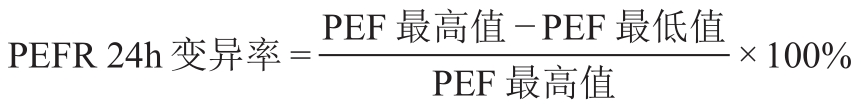
\includegraphics[width=2.85417in,height=0.36458in]{./images/Image00393.jpg}

\hypertarget{text00268.htmlux5cux23CHP9-3-2-3-2}{}
(2) 动脉血气分析:

所有收住院的哮喘患者都应及时检查动脉血气,PaCO\textsubscript{2}
正常或轻度升高,PaO\textsubscript{2} < 60mmHg,具有诊断意义。

\hypertarget{text00268.htmlux5cux23CHP9-3-2-3-3}{}
(3) 血清生化检查:

大约有1/10患者因使用激素、β\textsubscript{2}
受体激动剂、呼吸性碱中毒以及进食减少等因素而有不同程度的低钾血症。低钾增加了心律失常的危险性,应尽早发现并纠正。

\hypertarget{text00268.htmlux5cux23CHP9-3-2-3-4}{}
(4) X线检查:

急性重症哮喘本身胸部X线检查除双肺过度充气外一般无特殊发现,但如果患者情况许可有必要常规进行以除外气胸、纵隔气肿、肺不张或肺炎的存在。

\hypertarget{text00268.htmlux5cux23CHP9-3-2-3-5}{}
(5) 心电图:

急性重症哮喘有时很难与急性左心衰竭相鉴别,并发心律失常是导致哮喘症状不易缓解的原因之一。心电图、超声心动图有助于鉴别诊断,尤其是50岁以上的患者。

\paragraph{哮喘急性发作时病情严重程度分级}

中华医学会呼吸病学分会哮喘学组于2008年重新制订了支气管哮喘的定义、诊断、治疗和管理方案,并将哮喘急性发作的严重程度分为轻、中、重和危重四度,现将哮喘分度指标列于表\ref{tab95-1}。

\subsection{治疗}

哮喘急性发作的治疗取决于发作的严重程度以及对治疗的反应。治疗的目的在于尽快缓解症状、解除气流受限和低氧血症,同时还需要制订长期治疗方案以预防再次急性发作。

\subsubsection{紧急处理}

\paragraph{吸氧}

低氧血症是导致重症哮喘死亡的主要原因。在不给氧的情况下,使用β\textsubscript{2}
受体激动剂和茶碱类药物可进一步降低PaO\textsubscript{2}
。如果患者年龄在50岁以下,给予高浓度面罩吸氧(35\%~40\%)一般来说是安全的,单纯重症哮喘不同于慢性支气管炎、肺气肿急性发作,很少由于缺氧得到纠正而使通气不足,即使已有高碳酸血症,其主要危险仍然来自低氧血症而不是二氧化碳潴留。给氧的目的是要将动脉血氧分压至少提高到60mmHg,如果可能应维持在75~105mmHg。入院后首次血气分析至关重要,并应严密随访以了解低氧血症是否得到纠正,高碳酸血症是否发生,从而相应调整吸氧浓度和治疗方案。

\paragraph{肾上腺皮质激素的应用}

急性重症哮喘诊断一旦成立应尽早使用激素,激素不但能抑制炎性过程及炎性介质释放,降低气道高反应性,缓解由炎症所致气道阻塞,而且还具有恢复β\textsubscript{2}
受体功能的作用,但激素药效发挥需要数小时,应与支气管解痉剂联合使用。严重的急性发作或口服激素不能耐受时,可采用静脉注射或滴注,如甲泼尼龙80~160mg,或氢化可的松400~1000mg分次给药。地塞米松因半衰期较长,对肾上腺皮质功能抑制作用较强,一般不推荐使用。静脉给药和口服给药的序贯疗法有可能减少激素用量和不良反应,如静脉使用激素2~3天,继之以口服激素3~5天。口服激素与静脉给药疗效相当,副作用小。推荐用法:泼尼松龙30~50mg或等效的其他激素,每日单次给药。

\paragraph{短效}

β\textsubscript{2} -受体激动剂(SABA)
该类药物支气管解痉作用强、起效快(数分钟)但维持时间较短(4~6小时)常用的药物有沙丁胺醇(salbutamol)和特布他林(terbutalin)等。可通过压力定量气雾剂的储雾器给药,也可通过射流雾化装置给药。推荐在初始治疗时连续雾化给药,随后根据需要间断给药(每4小时1次)。目前尚无证据支持常规静脉使用β\textsubscript{2}
受体激动剂。

\begin{table}[htbp]
{\centering
\caption{哮喘急性发作时病情严重程度分级}
\label{tab95-1}
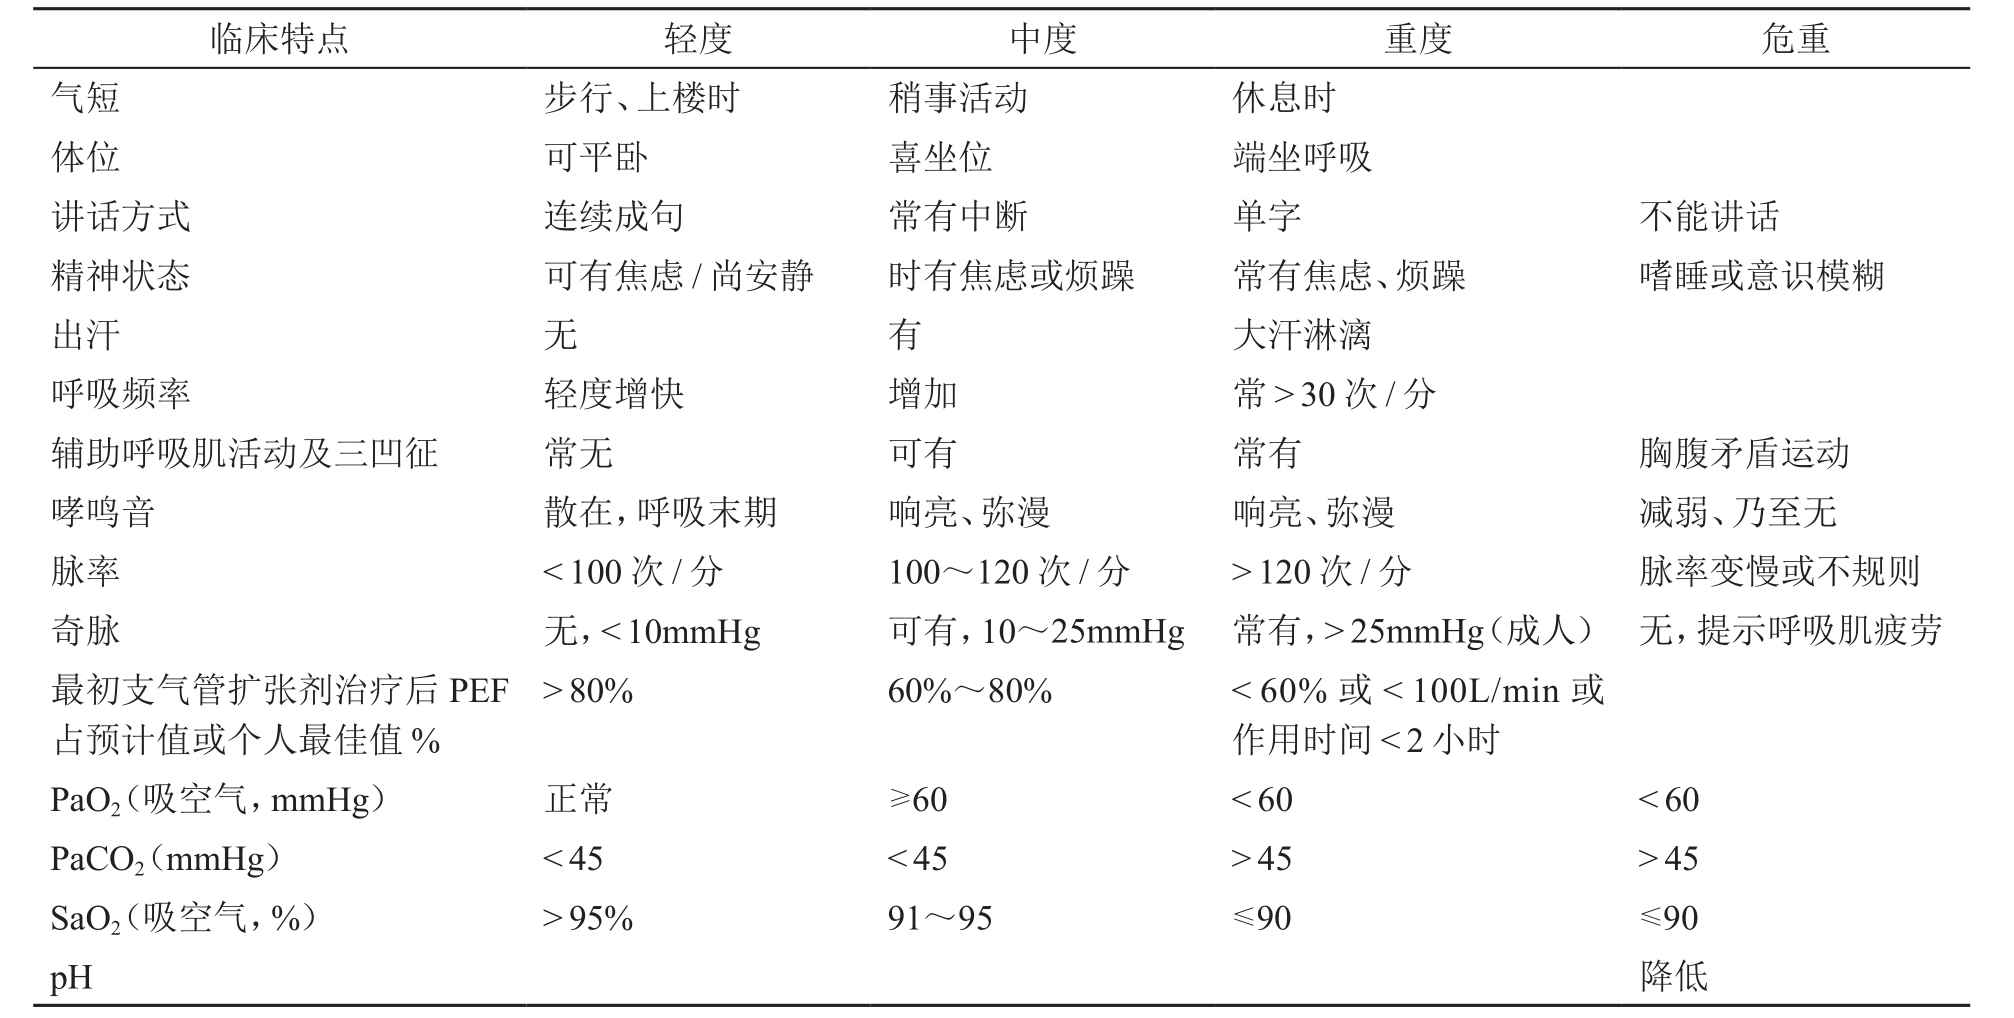
\includegraphics[width=6.70833in,height=3.38542in]{./images/Image00394.jpg}}

{\small 
注:只要符合某一严重程度的某些指标,而不需满足全部指标,即可提示为该级别的急性发作;1mmHg
= 0.098kPa
}
\end{table}



\paragraph{茶碱}

氨茶碱加入葡萄糖溶液中,缓慢静脉注射(注射速度不宜超过0.25mg/kg•min)或静脉滴注,适用于哮喘急性发作且近24小时内未用过茶碱类药物的患者。负荷剂量为4~6mg/kg,维持剂量为0.6~0.8mg/(kg•h)。由于茶碱的“治疗窗”窄,以及茶碱代谢存在较大的个体差异,可引起心律失常、血压下降、甚至死亡,在有条件的情况下应监测其血药浓度,及时调整浓度和滴速。茶碱有效安全血药浓度范围应在6~15mg/L。影响茶碱代谢的因素较多,如发热性疾病、妊娠,抗结核治疗可以降低茶碱的血药浓度;而肝脏疾患、充血性心力衰竭以及合用西咪替丁或喹诺酮类、大环内酯类等药物均可影响茶碱代谢而使其排泄减慢,增加茶碱的毒性作用,应引起临床医师的重视,并酌情调整剂量。

\paragraph{抗生素}

感染通常是哮喘急性加重的起因,而这种感染多半是由病毒引起,很少为细菌性,治疗重症哮喘常规使用抗生素并不能加快症状的缓解,如果确有细菌感染的依据或哮喘持续时间较长,使用抗生素仍有必要。有报道大环内酯类抗生素除具有抗感染作用外,对支气管哮喘也有一定的治疗作用。因为肺炎支原体和支原体感染对哮喘的发病起了一定的作用,此外,大环内酯类抗生素还有抗炎作用,可以升高茶碱的血浓度和刺激肾上腺皮质增生效应。

\paragraph{纠正水 、酸碱失衡和电解质紊乱}

重症哮喘,尤其是哮喘持续状态的患者,由于长时间的过度通气和进食减少容易形成脱水、气道分泌物浓缩形成痰栓,导致气道阻塞是哮喘死亡的主要原因之一,所以充分水化在治疗急性重症哮喘中占有不可忽视的地位,此时如患者心脏情况许可,每日适当补充液体,有助于纠正脱水、稀释痰液和防治痰栓形成。每日静脉补液量2500~3000ml。但对临床上无明显脱水的哮喘患者,则应避免过量补液,过多的补液并不能降低呼吸道分泌物的黏稠度,也不可能增加分泌物的清除,反而可造成血管内静水压的增加,降低血浆胶体渗透压,增加肺水肿的危险。尤其在哮喘急性发作的情况下,胸腔内的负压急剧增加,更易造成液体渗出的增加。重症哮喘患者由于抗利尿激素分泌增多,可出现低钾、低钠,如补液量过多可加重低钾、低钠,故大量补液时更应注意防止电解质紊乱。

重症哮喘患者由于缺氧、呼吸困难、呼吸功的增加等因素使能量消耗明显增加,往往合并代谢性酸中毒。由于严重的气道阻塞造成CO\textsubscript{2}
潴留,又可伴发呼吸性酸中毒。在酸血症的情况下,细支气管和肺血管发生痉挛,使气道阻力和通气/血流比例失调加剧。此外,在酸血症的情况下,许多支气管扩张剂均不能充分发挥疗效,故及时纠正酸中毒尤为重要。临床上通常把pH低于7.2作为补碱指征。但补充碳酸氢钠中和氢离子后可生成CO\textsubscript{2}
,从而加重CO\textsubscript{2}
潴留。所以,临床上以呼吸性酸中毒为主的酸血症,应以改善通气为主。如pH失代偿明显、且不能在短时间内迅速改善通气,以排出CO\textsubscript{2}
,则可补充少量5\%碳酸氢钠40~60ml,使pH升高到7.2以上,以代谢性酸中毒为主的酸血症可适当增加补碱量。

\subsubsection{紧急处理后病情监测和治疗}

在紧急处理后1~2小时,应重复PEFR检查,然后每日测量3~4次,并以表格记录。如治疗有效PEFR值会逐渐增加,PEFR昼夜变异率在起初会有所增大,但会随气道阻塞的改善而逐渐缩小,如PEFR变异率大幅度波动持续,意味着病情不稳定,需要继续严密监护和延长紧急治疗方案。动脉血气分析在紧急处理后1~2小时亦有必要重复以确定吸氧浓度使动脉血氧分压维持在60mmHg以上,氧分压恢复到正常水平的速度要比患者自觉症状和PEFR的恢复慢,一般需要数天甚至数周。如果患者自觉症状和客观测量的数据证实病情已有明显好转,在紧急处理后48~72小时,可将静脉注射激素和氨茶碱改为口服泼尼松45mg每日1次和氨茶碱控释片0.3g,每12小时1次,改雾化吸入β\textsubscript{2}
受体激动剂为定量气雾吸入或口服。约1/3~1/2的急性重症哮喘患者可在1~3天内迅速恢复,但多数患者需要1周或更长。经紧急处理后24小时如症状仍无缓解趋势,可适当加大雾化吸入沙丁胺醇的剂量和增加吸入频率,另可加用异丙托溴铵(异丙阿托品,ipratropine)500μg雾化吸入,每4小时1次。

\subsubsection{机械通气的应用}

对于常规药物治疗症状持续不缓解的重症哮喘,机械通气是十分有效的治疗手段,可先采用经鼻(面)罩无创机械通气,若无效应及早行气管插管机械通气。尽管只有大约1\%的重症哮喘需要进行人工通气,但是未能及时实施是造成哮喘死亡的原因之一,在呼吸、心跳停止前使用其预后要比呼吸、心跳停止后好而且使用周期短。多数作者认为重症支气管哮喘患者进行机械通气治疗可以达到下述目的:①迅速纠正严重的低氧血症和高碳酸血症,以及由此产生的一系列对机体的损害;②为支气管舒张剂等药物综合治疗取得疗效赢得时间;③让疲劳的呼吸肌得到充分的休息和恢复。

\paragraph{机械通气的适应证}

①意识进行性恶化,患者出现谵妄、昏迷,不能有效保护自身气道的通畅;②呼吸困难进行性加重,自主呼吸微弱甚至停止;③呼吸肌衰竭,导致通气不足、二氧化碳潴留,PaCO\textsubscript{2}
≥45mmHg;④经过积极、充分、全面的药物治疗,病情无好转仍呈进行性恶化趋势。其中,①、②条属绝对适应证,必须尽快行气管插管机械通气治疗,③、④条为相对适应证,需结合实际情况而定。临床具体应用时要灵活掌握,强调动态观察,适应证可适当放宽,估计病情发展机械通气治疗不可避免的患者,争取早插管、早拔管,减少并发症及死亡率。

\paragraph{气管插管的时机}

决定气管插管的一个重要因素是看患者的临床状态以及对治疗的反应,若在强有力的解痉平喘治疗下,病情仍进行性加重,患者表现为极度疲劳、呼吸频率下降、说话困难、意识状态不佳,不能自行排痰,即使其CO\textsubscript{2}
不高,pH也在可接受范围,也应立即进行气管插管机械通气。

\paragraph{人工气道的方式}

常用人工气道方式有经口和经鼻气管插管,支气管哮喘进行人工通气时,多可在72小时内撤机,现多主张采用经口气管插管,避免使用经鼻插管,哮喘患者常有鼻息肉和鼻窦疾病,使经鼻插管发生困难或插管时发生鼻腔大出血。经口插管应选用管径较大的8mm气管插管,以减少无效腔和阻力,方便吸痰。

\paragraph{机械通气初始参数的设置}

见表\ref{tab95-2}。

\begin{table}[htbp]
\centering
\caption{急性重症哮喘患者机械通气初始参数}
\label{tab95-2}
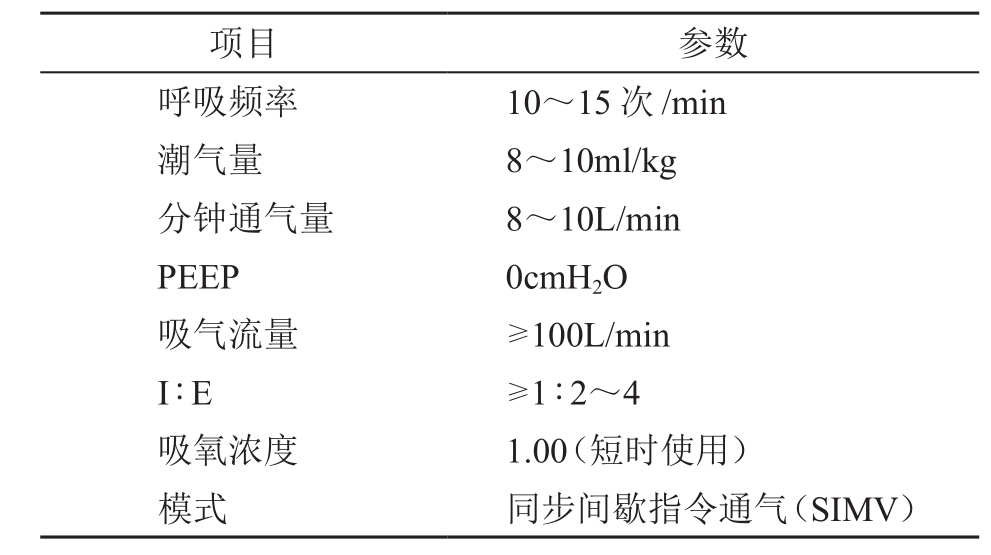
\includegraphics[width=3.29167in,height=1.83333in]{./images/Image00395.jpg}
\end{table}

出于对过高吸气峰压所造成严重损害的担忧,支气管哮喘患者进行机械通气治疗时,遵循“保证足够氧合而限制气道峰压”的原则,采取“控制性低通气(controlled
hypoventilation)”或“允许性高碳酸血症”(permissive
hypercarbia,PHC)通气策略。在机械通气的初期,参数设置提倡使用相对较小的潮气量(8~10ml/kg),保证吸气峰压低于40~50cmH\textsubscript{2}
O,较小的分钟通气量(8~10L/min),使血的碳酸控制在可接受水平。较高的吸气流速(100L/min)和较高的吸呼比(1∶2~4)可延长呼气时间以减少功能残气量和内源性PEEP。低氧血症在短时间内可通过提高FiO\textsubscript{2}
来实现,为迅速缓解缺氧,FiO\textsubscript{2}
可超过60\%,甚至短时间(30分钟以内)吸纯氧。高FiO\textsubscript{2}
和大通气量对过强的自主呼吸也有抑制作用,使之易于与机械通气同步。长时间持续机械通气时,为避免发生氧中毒,FiO\textsubscript{2}
应小于50\%。初期不主张使用PEEP,因为PEEP可加重肺泡过度充气,有导致气压伤的危险。

机械通气模式应根据患者意识状态、自主呼吸频率与深度情况而定。对于无自主呼吸患者,可采用控制通气模式(VC)。自主呼吸过分亢进,难以与机械通气同步的患者,也可先经药物抑制自主呼吸后再采用上述通气方式。对于自主呼吸节律平稳的患者应采用同步间歇指令通气(SIMV)或压力支持通气(PSV),机控通气频率和支持压力水平的设定应根据患者吸气肌功能情况及病情、病程来调整,应由大到小逐渐降低,直至脱离呼吸机。

对于部分中度支气管哮喘患者,在自主呼吸条件下,可采用经鼻面罩持续气道正压(CPAP)进行无创通气,可起到机械性扩张支气管和缓解喘息症状的目的。

\paragraph{PEEP的应用}

危重哮喘患者肺充气过度,在呼气末期由于呼气肌收缩使胸腔内压加大,气道易陷闭,造成气体滞留,呼气末肺容量增加,肺弹性回缩力增加,在肺泡内产生正压,称为内源性呼气末正压(PEEPi)。当患者吸气时,为克服PEEPi,需增加吸气肌做功。采用PEEP保持呼气末气道内正压,可扩张气道、降低吸气阻力,减少吸气肌的负荷做功,同时可避免由于进一步肺充气过度所产生的PEEPi,改善通气/血流比值。PEEP本身并不构成通气模式,它是一种辅助功能,可应用于PSV、SIMV等各种通气模式中。在初期设置参数和模式使用后,患者仍有显著的呼吸困难或仍需要大于50\%
FiO\textsubscript{2} 才能将SaO\textsubscript{2}
维持在90\%以上,可考虑使用PEEP。机械通气之初可逐步增加PEEP直至出现明显机械性气道扩张作用,如能监测PEEPi,PEEP应调至低于PEEPi的水平。为避免过高PEEP对循环系统的不良影响,最大值不要超过20cmH\textsubscript{2}
O。特别应当注意的是,当治疗有效、气道阻力下降后应及时降低PEEP,以减少气压伤发生的机会。

\paragraph{镇静剂与肌松剂的应用}

重症支气管哮喘患者在进行气管插管机械通气的时候,如果出现患者躁动不安、严重人机对抗,致使通气量严重不足、缺氧加重时可考虑选用镇静剂及肌松剂以促进人机配合,减少患者呼吸做功,降低气道峰压。但如果患者神志清楚,应尽量告知患者机械通气的必要性,以取得患者自主呼吸与通气机的配合,避免使用镇静剂或肌松剂,从而可尽早脱离机械通气。

\hypertarget{text00268.htmlux5cux23CHP9-3-3-3-6-1}{}
(1) 镇静剂的应用:

地西泮(安定)为临床常用的镇静剂之一,具有镇静、催眠和中枢性骨骼肌松弛作用,且能增强箭毒及三碘季胺酚的肌肉松弛作用,大剂量可抑制呼吸,常规用量为10mg静推,4小时可重复一次,该药在体内有蓄积作用。

\hypertarget{text00268.htmlux5cux23CHP9-3-3-3-6-2}{}
(2) 肌松剂的应用:

如给予镇静剂后仍不能消除患者自主呼吸与通气机之间的拮抗,此时可加用肌松剂。肌松剂的主要作用是干扰神经肌肉接头处的神经冲动传导过程,致使骨骼肌松弛。推荐使用非去极化剂类神经肌肉阻断剂,如泮库溴铵(pancuronium,潘龙),静脉注射后3~4分钟后即可显效,持续时间为30分钟左右,一般初量为0.08~0.1mg/kg体重,维持剂量0.01~0.02mg/kg。维库溴铵(vecuronium,万可松)是近年来应用于临床较理想的非去极化型肌松剂,不诱发组胺释放,无积蓄作用,初量为0.08~0.1mg/kg体重,1分钟内显效,维持时间15~30分钟,维持剂量0.01~0.015mg/kg体重,随着剂量增加,作用持续时间延长。

\subsubsection{氦-氧混合气体吸入}

氦为低质量惰性气体,其质量为空气的0.14倍,为氧的0.12倍。哮喘患者气流速度增高,近端气道以涡流为主。在涡流情况下气道两端的压力消耗(△P)可用以下公式表示:△P
= KρL/πr\textsuperscript{2} × V\textsuperscript{2}
,式中L为气道长度,r为半径,V为流速,K为常数,ρ代表气体的质量。也就是说△P与ρ成正比。另根据涡流系数原理,氦气比空气不易产生涡流。根据这些道理,吸入氦-氧混合气体比呼吸空气或吸入氧气时气道阻力要明显降低,结果减少了呼吸功氧耗量、二氧化碳产量,可防止呼吸肌疲劳的发生。氦气使二氧化碳弥散较氮氧混合气的CO\textsubscript{2}
弥散快4~5倍,又可使吸入气体在肺内分布均匀,有助于改善通气/血流比值失调。行此疗法时FiO\textsubscript{2}
在25\%~40\%,流量为12L/min,据报道多数患者面罩吸入He-O\textsubscript{2}
混合气体后20分钟就可有明显好转,与药物治疗合用,可能使某些患者避免机械通气。

\subsubsection{机械通气的撤离}

哮喘的机械通气治疗需时较短,大部分在72小时之内,一般不会发生撤机困难。当患者哮鸣音明显减少,呼吸音趋于正常,神志清醒、气道阻力(某些呼吸机附有监测装置)接近正常,即可试验停机。停止机械通气1小时,低流量吸氧条件下(FiO\textsubscript{2}
小于30\%)能维持PaO\textsubscript{2} > 65mmHg,PaCO\textsubscript{2} <
45mmHg,患者没有出现其他不适,即可拔除人工气道。对于体弱、一般状态差或有并发症发生的患者,撤机过程可能长一些,可经过PSV、SIMV或PSV加SIMV的方式来过渡,并注意能量与蛋白质的补充。

\protect\hypertarget{text00269.html}{}{}

\hypertarget{text00269.htmlux5cux23CHP9-3-4}{}
参 考 文 献

1. 中华医学会呼吸病学分会哮喘学组.支气管哮喘防治指南(2008).

2. 蔡柏蔷 ,李龙芸.协和呼吸病学.中国协和医科大学出版社,2005:835-873.

3. 刘又宁 .机械通气与临床.第2版.北京:科学出版社,1998:415-421.

\protect\hypertarget{text00270.html}{}{}

\chapter{自发性气胸}

气胸(pneumothorax)系肺组织及脏层胸膜破裂,或胸壁及壁层胸膜被穿透,空气进入胸膜腔,形成胸膜腔积气和肺脏萎缩。可分成自发性、创伤性和医源性三类。医源性气胸由诊断和治疗操作所致。导致医源性气胸的原因有经胸腔细针吸引(占24\%~36\%),锁骨下静脉穿刺(占22\%~23\%)和胸腔穿刺(占20\%~31\%)。机械通气也是医源性气胸的致病原因,约占所有医源性气胸的7\%。创伤性气胸是胸壁的直接或间接损伤所致。胸部的穿透性损伤常引起创伤性气胸,而闭合性胸部创伤,由于胸部受压,支气管断裂,食管破裂或肋骨骨折损伤胸膜等也可导致气胸。而在没有创伤或人为因素的情况下,肺组织及脏层胸膜自发性破裂,空气进入胸膜腔,称为自发性气胸(spontaneous
pneumothorax,SP)。SP又可分为原发性气胸(primary
SP)和继发性气胸(secondary
SP)两型,前者又称特发性气胸,指肺部X线检查无明显病变的健康者所发生的气胸,多见于20~40岁的青壮年,男性较多;后者继发于肺脏各种疾病,常见于40岁以上者。本章着重论述自发性气胸。

\subsection{病因与发病机制}

正常情况下胸膜腔内没有气体,这是由于毛细血管血中各种气体分压的总和仅为706mmHg,比大气压低54mmHg。呼吸周期胸膜腔内压均为负压,系胸廓向外扩张,肺向内弹性回缩对抗产生的。胸膜腔内出现气体常见于两种情况:①肺泡与胸腔之间产生破口,气体将从肺泡进入胸膜腔直至压力差消失或破口闭合;②胸壁创伤产生与胸膜腔的交通,也出现同样的结果。少见的是胸膜腔内有产气的微生物存在。

原发性气胸多见于瘦高体型的男性青壮年,常规X线检查肺部无显著病变。其发病机制一般认为是多位于肺尖部位的胸膜下肺大疱(subpleural
bleb,SB)破裂所致。对于SB的形成,与吸烟、身高和小气道炎症可能有关,也可能系先天性弹力纤维发育不良,肺泡壁弹性减退、扩张后形成大泡;或系非特异性炎症瘢痕引起肺表面微小气肿疱。Vanderscheren根据胸腔镜下肺泡病变与胸膜粘连的情况,将SP在临床上分为4级:Ⅰ级为特发性气胸,内镜下观察肺组织无明显异常;Ⅱ级为气胸伴有脏层、壁层胸膜增厚;Ⅲ级为脏层胸膜大疱和直径<
2cm的肺大疱;Ⅳ级有多个直径>
2cm的肺大疱。本分级方法对指导选择合理的治疗方法有临床实用价值。有学者强调胸膜间皮细胞在SP发生中起重要作用:认为SP的形成并不一定要以肺大疱破裂为前提,而可能是由于胸膜间皮细胞稀少或完全缺乏,在肺内压增高的情况下,空气通过大疱壁的裂孔进入胸膜腔引起气胸。此外,在本病的病因中,尚有“新膜理论”(neomembrane
theory)、侧支通气障碍机制和大气污染学说等。此型气胸患者的肺组织破裂瘘孔或细支气管胸膜瘘孔大多数形成闭合性SP,较少形成开放性SP,更少形成张力性SP。

继发性气胸的发生机制是在其他肺部疾病基础上形成肺大疱或直接损伤胸膜所致。常见为慢性阻塞性肺气肿或肺弥漫性纤维化疾病(矽肺、慢性肺结核、弥漫性肺间质纤维化、囊性肺纤维化等)并发代偿性肺大疱时,由于其引流的小气道炎性狭窄,肺泡内压力急骤升高,导致肺大疱破裂,引起气胸。金葡菌、厌氧菌、革兰阴性杆菌引起的肺化脓性、坏死性炎症亦可溃破入胸腔,形成脓气胸。肺癌合并气胸的机制为:①癌肿结节形成活瓣,造成支气管腔不完全阻塞,远端肺泡过度膨胀,破入胸膜腔;②癌肿完全堵塞支气管,引起肺不张,邻近肺组织代偿性肺气肿,气肿疱破裂而致气胸;③肺癌远端阻塞性肺炎,脓肿形成,坏死后破入胸膜腔;④空洞型肺癌坏死破入胸膜腔;⑤周围型肺癌直接侵犯脏层胸膜,形成支气管胸膜瘘;⑥放射治疗后肿瘤坏死,或放射性肺炎致肺纤维化、瘢痕牵拉可致肺大泡形成或破裂。肺囊肿、肺结核空洞亦可侵犯胸膜,引起气胸。其他疾病还有结节病、组织细胞增生症X、硬皮病、嗜酸性粒细胞肉芽肿、胆汁性肝硬化、类风湿关节炎等。与月经周期有关的反复发作性气胸------月经性气胸,约占女性SP患者的5.6\%,以30岁以上女性多见,常在月经24~72小时内发生,气胸多发生在右侧。其发生的机制可能是肺、胸膜或横膈的子宫内膜移位,使:①SB自发性破裂;②前列腺素使细支气管收缩,管腔部分阻塞使远端肺泡过度充气后破裂;③子宫和输卵管的空气,经过右横膈小孔进入胸腔。继发性气胸常由于:①部分患者因肺原有疾病已和壁层胸膜粘连,当SP形成后,患部脏、壁层胸膜因粘连于胸壁,而牵拉瘘孔部位的肺组织不向肺门部压缩,瘘孔亦被牵拉而开放,或形成活瓣;②部分患者因患病的肺组织破裂形成SP故难愈合;③少数患者肺内病变的支气管管腔狭窄、半阻塞而形成类似活瓣的作用。故继发性SP多数患者形成开放性或张力性SP,仅少数为闭合性。

脏层胸膜破裂或胸膜粘连带撕裂,如其中的血管破裂可形成自发性血气胸。航空、潜水作业而无适当防护措施时,从高压环境突然进入低压环境,以及机械通气压力过高时,均可发生气胸。抬举重物等用力动作,咳嗽、喷嚏、屏气或高喊大笑等常为气胸的诱因;但不少患者在正常活动或安静休息时发病。

气胸时失去了负压对肺的牵引作用,甚至因正压对肺产生压迫,使肺失去膨胀能力,表现为肺容积缩小、肺活量减低、最大通气量降低的限制性通气功能障碍。由于肺容积缩小,初期血流量并不减少,产生通气/血流比例下降,导致动静脉分流,出现低氧血症。大量气胸时,由于失去负压吸收静脉血回心,甚至胸膜腔内正压对血管和心脏的压迫,使心腔充盈减少,心搏出量降低,引起心跳加快、血压降低,甚至休克。张力性气胸可引起纵隔移位,致循环障碍,甚或窒息死亡。

气胸易于复发,且在每次发作后随着复发次数的增多,发作频率会增加。Gaensler统计,第二次发作的复发机会是50\%,第三次发作的复发机会是62\%,第四次发作的复发机会是80\%。继发性SP的复发率约为50\%。

\subsection{诊断}

\subsubsection{临床表现特点}

气胸病情的轻重与有无肺基础疾病及功能状态、气胸发生的缓急、胸腔内积气量及其压力高低三个因素有关。若原已存在严重肺功能减退,即使气胸量小,也可有明显的呼吸困难;青年人即使肺压缩80\%以上,有的症状也可以很轻。起病前部分患者可能有抬举重物用力过猛、咳嗽、喷嚏、屏气或高喊大笑等诱因,但多数患者在正常活动或安静休息时发病。

大多数起病急骤,典型症状为突发性胸痛,继之有胸闷和呼吸困难,并可有刺激性咳嗽。胸痛是由于胸膜牵拉、撕裂的结果,其性质如刀割或针刺样锐痛,并随深呼吸而加剧,以后逐渐转为持续性隐痛;疼痛部位位于患侧腋下、锁骨下及肩胛下,有时可向同侧肩背或上腹部放射。继胸痛后常有胸闷或呼吸困难。少数患者可有咳嗽气喘,咳嗽呈刺激性(因气体刺激胸膜所致)。少量气胸无明显症状或先有气急后逐渐平稳;大量气胸时,患者感胸闷、气短、呼吸困难,不能平卧。继发性气胸由于肺部病变广泛,肺功能减退,并发气胸往往气急显著,伴发绀;张力性SP常呈进行性严重呼吸困难,有窒息感,甚至发生呼吸衰竭和休克,若不及时抢救,常引起死亡。少量气胸时体征不明显。气胸在30\%以上,患侧胸部膨隆,呼吸运动减弱,叩诊呈鼓音,语颤及呼吸音减弱或消失。大量气胸可使心脏、气管向对侧移位、有水气胸时可闻及胸内溅水声。少量胸腔积液常是由于空气刺激胸膜产生的渗出液,但也可能由于气胸导致胸膜粘连带撕裂引起血气胸。

由于肺泡破裂逸出的气体进入肺间质,形成间质性肺气肿。肺间质内的气体沿血管鞘可进入纵隔,甚至进入胸部或腹部皮下组织,导致皮下气肿。张力性SP抽气或闭式引流后,亦可沿针孔或切口出现胸壁皮下气肿,或全身皮下气肿及纵隔气肿。气体积聚在纵隔间隙可压迫纵隔大血管,出现干咳、呼吸困难、呕吐及胸骨后疼痛,并向双肩或双臂放射。疼痛常因呼吸运动及吞咽动作而加剧。患者发绀、颈静脉怒张、低血压、心浊音界缩小或消失、心音遥远,心尖部可听到与心跳同步的“卡嗒”声(Hamman's征)。皮下气肿及纵隔气肿随胸腔内气体排出减压而自行吸收。若纵隔气肿张力过高影响呼吸及循环,可作胸骨上窝切开排气。

\subsubsection{辅助检查}

\paragraph{X线检查}

X线检查(包括透视、摄片)显示气胸征是确诊的依据。它可以显示肺脏萎缩的程度、肺内病变情况以及有无胸膜粘连、胸腔积液和纵隔移位等。气胸的典型X线表现为外凸弧形的细线条形阴影,称为气胸线,线外透亮度增高,无肺纹理,线内为压缩的肺组织。大量气胸时,肺脏向肺门回缩,呈圆球形阴影。大量气胸或张力性气胸常显示纵隔和心脏向健侧移位。合并纵隔气肿在纵隔旁和心缘旁可见透光带。少量气胸常局限于肺尖,常被骨骼掩盖,嘱患者深呼气,使萎缩的肺更为缩小,密度增高,与外带积气透光区呈更鲜明对比,从而显示气胸带。局限性气胸在后前位X线检查时易遗漏,需在X线透视下转动体位方能见到气胸。但X线检查的缺点是小量气胸的患者不敏感,对某些肺大泡等患者有时不易鉴别。

计算肺压缩面积,可在后前位胸片或透视下,取肺门为中心作三条线,一条经第一前肋下缘达外胸壁,第二条自肺门水平向外达胸壁,第三条自肺门斜行向下达肋膈角,每条线全长为100\%,分别计算出三条线上肺萎缩的百分比,然后以下列公式计算:压缩全肺\%=上+中+下/3。

此外,还可从后前位X线胸片判断气胸容量,即:侧胸壁至肺边缘的距离为1cm时,约占单侧胸腔容量的25\%左右,2cm时约50\%,故从侧胸壁与肺边缘的距离≥2cm为大量气胸,<
2cm为小量气胸。如从肺尖气胸线至胸腔顶部估计气胸的大小,距离≥3cm为大量气胸,<
3cm为小量气胸。

\paragraph{CT扫描}

CT扫描表现为胸膜腔内出现极低密度的气体影,伴有肺组织不同程度的萎缩改变。CT对于小量气胸、局限性气胸以及肺大疱与气胸的鉴别比X线胸片更敏感和准确。CT还可鉴别位于纵隔旁的SP与纵隔气肿以及肺气囊,对有广泛皮下气肿存在的患者,CT检查常可发现X线平片阴性的SP存在。

\paragraph{胸腔镜检查}

为一创伤性的检查方法,最大益处在于可以较为容易地发现气胸的病因。其优点是:①损伤小,胸壁切口1~2cm;②操作灵活,可达叶间裂、肺尖、肺门,几乎没有盲区;③观察仔细,可见脏层胸膜下的微小肺大疱;④可重复进行,必要时镜下取标本。因此,可使90\%
的SP患者明确病因。但有广泛胸膜粘连、凝血机制障碍、严重心肺功能不全、剧烈咳嗽或极度衰竭不能耐受检查者、严重的肺动脉高压或肺静脉淤血等禁用。

\subsubsection{临床分型}

根据脏层胸膜破口的情况及其发生后对胸腔内压力影响,将SP分为闭合性(单纯性)气胸、张力性(高压性)气胸和开放性(交通性)气胸三种类型,见表\ref{tab96-1}。胸膜腔抽气测压可用于判定气胸的类型,用2ml空针试压,在吸胸腔气体约1ml后观察时,开放性者针栓随患者呼吸在原处来回移动,张力性者针栓随呼吸外移,如气体又随呼吸回入胸腔则为闭合性。但这三种类型SP在病情发展过程中可以相互转换,因此,对于任何类型的SP,均应严密观察,以及时发现病情的转变。

\begin{table}[htbp]
\centering
\caption{自发性气胸的分型}
\label{tab96-1}
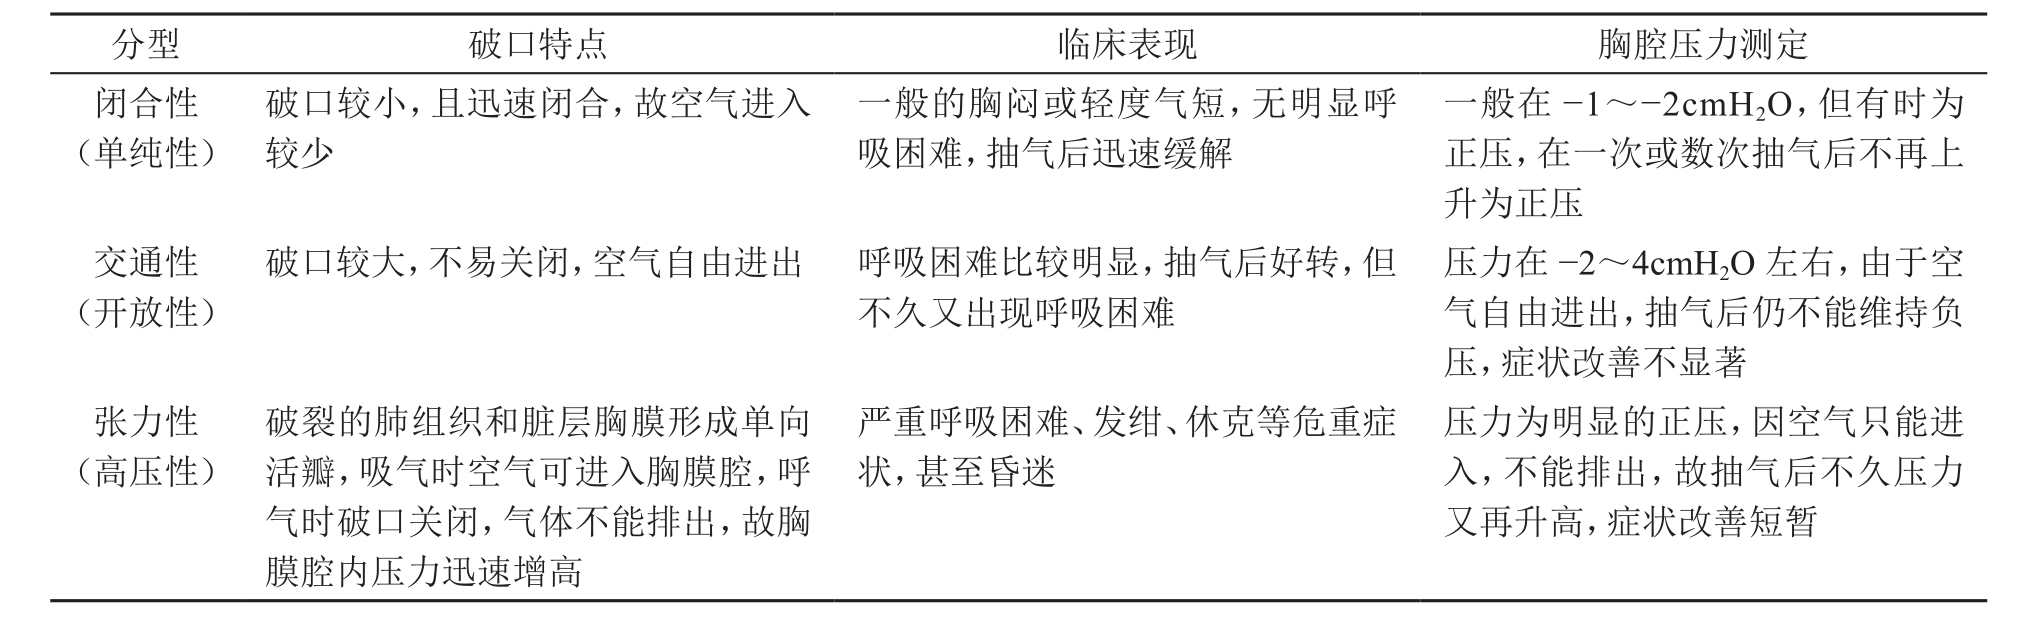
\includegraphics[width=6.72917in,height=2.04167in]{./images/Image00396.jpg}
\end{table}

为了便于临床观察和处理,尚可根据临床表现把SP分为稳定型和不稳定型,符合下列所有表现者为稳定型,否则为不稳定型:呼吸频率<
24次/分;心率60~120次/分;血压正常;呼吸室内空气时SaO\textsubscript{2}
> 90\%;两次呼吸间说话成句。

\subsubsection{鉴别诊断}

依据典型症状和体征,一般诊断并不困难,局限性少量气胸或原有肺气肿者,须借助X线、CT检查等来帮助确诊。若病情十分危重无法搬动作X线、CT等检查时,应当机立断在患侧胸腔体征最明显处试验穿刺,如抽出气体,可证实气胸的诊断。主要应注意鉴别的疾病有:

\paragraph{急性心肌梗死}

患者亦有急起胸痛、胸闷,甚至呼吸困难、休克等表现,但常有高血压、冠心病史,心电图、X线、肌钙蛋白I及血清酶学检查等可有助于鉴别诊断。偶有左侧气胸在卧位时亦出现类似心肌梗死的心电图改变,但患者直立位的心电图正常。

\paragraph{支气管哮喘和慢性阻塞性肺疾病(COPD)}

两者均有不同程度的气急和呼吸困难,体征亦与SP相似,但COPD患者的呼吸困难是长期缓慢加重的,支气管哮喘患者有多年哮喘反复发作史。当哮喘和肺气肿患者呼吸困难突然加重且有胸痛、冷汗、烦躁,支气管舒张剂、抗感染药物等治疗效果不好,且症状加剧,应考虑并发气胸的可能。胸部X线、CT检查可作出诊断。

\paragraph{肺血栓栓塞症}

有胸痛、呼吸困难和发绀等酷似SP的临床表现,但患者常有咯血和低热,并常有下肢或盆腔栓塞性静脉炎、骨折、严重心脏病、房颤病史,或发生在长期卧床的老年患者。体检和X线、CT检查有助于鉴别。

\paragraph{肺大疱}

位于肺周边的肺大疱,尤其是巨型肺大疱易被误诊为气胸。肺大疱通常起病缓慢,呼吸困难并不严重,而气胸症状多突然发生。影像学上,肺大疱气腔多呈圆形或卵圆形,疱内有细小的条纹理,为肺小叶或血管的残遗物。肺大疱向四周膨胀,将肺推向肺尖区、肋膈角或心膈角。而气胸则呈胸外侧的透光带,其中无肺纹理可见。从不同角度作胸部透视,可见肺大疱为圆形透光区,在肺大疱的边缘看不到发丝状气胸线。肺大疱内压力与大气压相仿,抽气后,肺大疱容积无明显改变。经较长时间观察,肺大疱很少有变化,而气胸形态则随时日而变小,最后消失。如误对肺大疱抽气测压,甚易引起气胸。

\paragraph{其他}

如消化性溃疡穿孔、膈疝、胸膜炎和肺癌等,有时因有急起的胸痛、上腹痛和气急等,亦应与SP注意鉴别。

\subsection{治疗}

SP的治疗目的是促进患侧肺复张、消除病因及减少复发。具体措施有保守治疗、胸腔减压、经胸腔镜手术或开胸手术等。应根据气胸的类型与病因、发生频次、肺压缩程度、病情状态及有无并发症等适当选择。持续性气胸(系指SP经肋间切开水封瓶引流或加用持续负压吸引,仍然漏气超过14天者)或复发性气胸(指单侧气胸发作超过2次或双侧性气胸发作3次以上者)(这两种气胸通称为顽固性气胸)均提示肺内有不可逆的病理改变,应积极治疗,预防复发是十分重要的。

影响肺复张的因素包括患者年龄、基础肺疾病、气胸类型、肺萎陷时间长短以及治疗措施等。老年人肺复张时间通常较长;交通性气胸较闭合性气胸需时长;有基础肺疾病、肺萎陷时间长者肺复张时间亦长;单纯卧床休息肺复张时间显然较胸腔闭式引流或胸腔穿刺抽气为长。有支气管胸膜瘘、脏层胸膜增厚、支气管阻塞者,均妨碍肺复张,并易导致持续性气胸。

\subsubsection{保守治疗}

主要适用于稳定型小量气胸、首次发生的症状较轻的闭合性气胸。应严格卧床休息,酌情予以镇静、镇痛等药物。剧烈咳嗽者口服喷托维林25mg,每日3次,或可待因0.03g,每日3次。支气管痉挛者给予氨茶碱0.25g加入葡萄糖液40ml静脉缓慢注射,或沙丁胺醇(舒喘灵)气雾剂吸入。保持大便通畅。高浓度吸氧治疗。由于胸腔内气体分压和肺毛细血管内气体分压存在压力差,每日内可自行吸收胸腔内气体容积的1.25\%~1.8\%;经鼻导管或面罩持续高浓度(氧流量3L/min)吸氧可使气胸患者气体吸收率提高达4.2\%,较一般卧床休息肺复张所需时间显著缩短。其机制是提高血中PO\textsubscript{2}
,使氮分压(P\textsubscript{N}
)下降,从而增加胸膜腔与血液间的P\textsubscript{N}
差,促使胸膜腔内的氮气向血液转递(氮-氧交换),加快肺复张。保守治疗需密切监测病情改变,尤其在气胸发生后24~48小时内。同时重视肺基础疾病的治疗。如果患者年龄偏大,并有肺基础疾病如COPD,其胸膜破裂口愈合慢,呼吸困难等症状严重,即使气胸量较小,原则上不主张采取保守治疗。此外,气胸患者应常规使用抗生素治疗直至胸膜腔愈合为止,可选用青霉素、氨苄西林、氨基糖苷类、喹诺酮类、头孢菌素类等。

也可用超短波治疗肺压缩面积25\%以下的自发性气胸。剂量为温热量,每次25分钟,每日1次,6次为1个疗程。可使肺复张时间明显缩短,每日气体吸收率明显提高。其机制为:超短波可以增加气体分子的热运动,使气体膨胀,压力升高,肺毛细血管扩张,改善局部血液循环,有利于气体向血管内弥散,促进气体吸收。此外,超短波可使组织代谢加快,刺激结缔组织和肉芽组织生长,加速伤口愈合。

\subsubsection{排气疗法}

\paragraph{胸膜腔穿刺抽气法}

适用于小量气胸,呼吸困难较轻,心肺功能尚好的闭合性气胸患者。抽气可加速肺复张,迅速缓解症状。患者取坐位或仰卧位,在患侧胸部锁骨中线第2肋间或腋前线第4~5肋间处作为穿刺点,皮肤消毒后用气胸针或细导管直接穿刺入胸膜腔,随后连接于50ml或100ml注射器或人工气胸机抽气并测压,直到患者呼吸困难缓解为止。一般一次抽气量不宜超过1000ml或使胸膜腔压力降至“0”上下,每日或隔日抽气一次。对危及生命的张力性气胸的紧急处理,在没有条件的医疗单位或现场救治中,可用粗针头迅速刺入胸膜腔,以达到暂时减压的目的。亦可采用粗注射针,将针柄接扎上橡皮指套,指套末端剪一小口,针插进胸膜腔后,高压气体迅速自小口排出,到达负压时,指套囊即瘪塌,小口闭合,外界空气不能进入。此为临时性急救措施,此后仍应行胸腔水封瓶闭式引流。

\paragraph{胸腔闭式引流术}

适用于不稳定性气胸,呼吸困难明显,肺压缩程度较重,交通性和张力性气胸,反复发生气胸的患者。上述部位局部消毒、麻醉后,沿肋骨上缘平行作1.5~2.0cm皮肤切口,用套管针穿刺进入胸膜腔,拔去针芯,通过套管将灭菌胶管插入胸腔。亦可在切开皮肤后,垂直钝性分离皮下组织和肌层达胸膜后,以止血钳或刀穿破胸膜,将导管直接送入胸膜腔。一般选用胸腔引流专用的硅胶管,或外科胸腔引流管。16~22F导管适用于大多数患者,如有支气管胸膜瘘或机械通气的患者,应选择24~28F导管。导管固定后,另一端可连接Heimlich单向活瓣,或置于水封瓶的水面下1~2cm,使胸腔内压力保持在1~2cmH\textsubscript{2}
O以下,插管成功则导管持续溢出气泡,呼吸困难迅速缓解,压缩的肺可在数小时至数天内复张。对肺压缩严重、时间较长的患者,插管后应夹住引流管分次引流,避免胸腔内压力骤降产生肺复张后肺水肿。水封瓶应消毒应用,瓶内液体可用消毒清水或生理盐水,一般隔日更换一次消毒水封瓶。水封瓶一般放在病床边的地面上,并应避免将其提高到接近胸腔的水平。若水封瓶玻管与连接橡皮管畅通无阻,而无气泡逸出,且患侧肺呼吸音已恢复,可认为肺已复张;如经X线检查确认肺复张,则用止血钳夹住导管,观察24~48小时,复查如再无气胸的存在,则可拔管。有时虽未见气泡溢出,但患者症状缓解不明显,应考虑为导管不通畅或部分滑出胸膜腔,需及时更换导管或作其他处理。局限性气胸或有胸膜粘连者,应在X线透视定位下插管;液气胸需排气排液者,多选择上胸部插管引流,有时需置上、下两根引流管。

单纯水封瓶闭式引流系正压排气引流,胸膜腔内须达一定正压,气体才能排出(引流玻管没水不宜太深,一般在1~2cm)。此法简便易行,但排气有时不彻底,肺复张稍慢。有时为补救肺复张较慢的不足,于引流数天后,估计瘘孔已经闭合,可令患者轻轻咳嗽,使胸膜腔产生短暂正压,以利气体排出。若胸膜腔内气体迅速减少,说明瘘孔确已闭合;如虽有不少气体排出,但胸膜腔内气体不见减少,则提示瘘孔并未闭合,不宜令患者咳嗽排气,可继续行单纯水封瓶闭式引流。若应用胸腔水封瓶闭式引流2~3周左右仍溢出气泡者则考虑行药物粘连(见下述)。注药后由于瘘孔部位产生渗出、粘连、闭合,95\%以上患者均在1~2天将残留胸腔气体从水封瓶排出而肺全复张。对极少数患者肺复张较慢,在确定瘘孔已闭合和气道通畅后,则可行低的负压吸引,促使肺复张。

负压吸引水封瓶闭式引流是在水封瓶排气管中,安装一个压力调节瓶调节负压,压力调节管下端离水面8~12cm,即抽吸负压为8~12cmH\textsubscript{2}
O,最深不宜超过14cm。如有胸腔积液,可在水封瓶前加一个液体收集瓶,以便观察排液情况。如肺已完全复张,可试停负压吸引,夹住引流管让患者活动,观察48~72小时经透视或胸片证实气胸未再复发后,可拔除导管,伤口以蝶形胶布拉拢,纱布覆盖。

原发性SP经导管引流后,即可使肺完全复张;继发性SP常因气胸分隔,单导管引流效果不佳,有时需在患侧胸腔插入多根导管。双侧同时发生SP者,可在双侧胸腔插管引流。

\subsubsection{胸膜粘连术}

胸膜粘连术是将无菌的刺激性物质注入胸膜腔,诱发化学性胸膜炎,使脏层、壁层胸膜粘连,瘘孔闭合,消失胸膜腔间隙,使空气无处积存,从而治疗和避免气胸复发。该方法也谓之化学性胸膜固定术(pleurodesis)。主要适用于:①持续性或复发性SP患者;②有双侧自发性气胸史者;③合并肺大疱者;④肺功能低下,不能耐受胸科手术者。常用的胸膜粘连剂有滑石粉5g(或5\%悬液100ml)、四环素(红霉素)0.5g、硝酸银溶液(1‰
20~30ml)、樟脑油(1\%
10ml)等,由于滑石粉胸膜固定术SP复发率7\%~15\%,仅次于手术(0.6\%~2\%),故以滑石粉为首选。滑石粉5g用生理盐水60~100ml稀释后经胸导管注入胸膜腔,夹管1~2小时后引流。注入药物后,嘱患者多方向转动体位,以使注入物质均匀涂布在胸膜表面。为避免药物引起的局部剧痛,可先注入适量利多卡因,让患者转动体位,充分麻醉胸膜,15~20分钟后再注入药物。若一次无效,可重复注药。观察1~3天,经X线透视或照片证实气胸已吸收,可拔除引流管。此法成功率高。故有人主张在对SP患者胸腔闭式引流后,肺全复张的拔管前均行滑石粉注入胸腔(转动体位后引流出),以减少或防止SP复发。

\subsubsection{手术治疗}

经内科治疗无效的气胸可为手术的适应证,主要适用于长期气胸、血气胸、双侧气胸、复发性气胸、张力性气胸引流失败者、胸膜增厚致肺膨胀不全或影像学有多发性肺大疱者。手术治疗成功率高,复发率低。

\paragraph{胸腔镜}

在胸腔镜直视下对准肺大疱或破裂口,喷注纤维蛋白胶或快速医用ZT胶,使破口黏合;直视下粘连带烙断术促使破裂口关闭;或用Nd-YAG激光或二氧化碳激光烧灼<
2.0cm的肺大疱。电视胸腔镜(VATS)可行肺大疱结扎、肺段或肺叶切除,具有微创、安全等优点。

\paragraph{开胸手术}

近年来由于肺外科手术的进步,开胸处理SP已是较安全可靠的方法。外科手术可以消除肺的破口,又可从根本上处理原发病灶(如肺大疱、肺癌或结核空洞穿孔等),或通过手术以确保胸膜粘连。手术适应证为:

\hypertarget{text00270.htmlux5cux23CHP9-4-3-4-2-1}{}
(1) 复发性气胸:

尤其是合并胸腔感染者(如脓胸)。

\hypertarget{text00270.htmlux5cux23CHP9-4-3-4-2-2}{}
(2) 肺的原发性病灶需手术治疗者:

包括:①张力性气胸闭式引流失败者;②长期漏气所致肺不张者,或存在支气管胸膜瘘者;③大量血气胸;④双侧气胸(尤其是同时发生者);⑤胸膜增厚,或已有纤维膜形成使肺不能膨胀者;⑥自发性气胸伴有巨型肺大疱者;⑦特殊性气胸,如月经性气胸等;⑧青少年原发性气胸(因易复发,且可引起双侧气胸)。若患者X线胸片上见到多发性肺小疱则手术指征更强。

\protect\hypertarget{text00271.html}{}{}

\hypertarget{text00271.htmlux5cux23CHP9-4-4}{}
参 考 文 献

1. 陶仲为 .自发性气胸.中国实用内科杂志,2005,25(8):749

2. 陈灏珠 ,林果为.实用内科学.第13版.北京:人民卫生出版社,2009:1875

3. 陆再英,钟南山.内科学,第7版.北京:人民卫生出版社,2008:116

4. 俞森洋
,蔡柏蔷.呼吸内科主治医生660问.第2版.北京:中国协和医科大学出版社,2009:558

\protect\hypertarget{text00272.html}{}{}

\chapter{肺 炎}

肺炎(pneumonia)是指终末气道,肺泡和肺间质的炎症,可由病原微生物、理化因素、免疫损伤、过敏及药物所致。依病因分类细菌性肺炎是最常见的肺炎。现在主张凡未表明特定病因者,肺炎即指感染性的。感染性病原引起的肺炎常与肺部感染一词混用。严格地说肺部感染仅是一种病因分类上的表述,尚包括气道等部位的感染,不能用于疾病的诊断。

依解剖分类法可分为:①大叶性(肺泡性)肺炎:病原体先在肺泡引起炎症,经肺泡间孔(cohn孔)向其他肺泡扩散,致使部分或整个肺段、肺叶发生炎症改变。典型者表现为肺实质炎症,通常并不累及支气管。致病菌多为肺炎链球菌。X线胸片显示肺叶或肺段的实变阴影。②小叶性(支气管性)肺炎:病原体经支气管入侵,引起细支气管、终末细支气管及肺泡的炎症。常继发于其他疾病,如支气管炎、支气管扩张、上呼吸道病毒感染以及长期卧床的危重患者。其病原体有肺炎链球菌、葡萄球菌、病毒、肺炎支原体以及军团菌等。支气管腔内有分泌物,故常可闻及湿性啰音,无实变体征。X线显示为沿肺纹理分布的不规则斑片状阴影,边缘密度浅而模糊,无实变征象。肺下叶常受累。③间质性肺炎:以肺间质为主的炎症,可由细菌、支原体、衣原体、病毒或卡氏肺囊虫等引起。累及支气管壁及其周围组织,有肺泡壁增生及间质水肿,因病变仅在肺间质,故呼吸道症状较轻,异常体征较少。X线常表现为一侧或双侧肺下部的不规则条索状阴影,从肺门向外伸展,可呈网状,其间可有小片肺不张阴影。

依病因分类法可分为:①细菌性肺炎:可分为肺炎链球菌、金黄色葡萄球菌、甲型溶血性链球菌、肺炎克雷伯杆菌、流感嗜血杆菌、铜绿假单胞菌肺炎等。②非典型病原体所致肺炎:如军团菌、支原体和衣原体等。③病毒性肺炎:如冠状病毒、腺病毒、呼吸道合胞病毒、流感病毒、麻疹病毒、巨细胞病毒、单纯疱疹病毒等。④真菌性肺炎:如白念珠菌、曲霉、放线菌等。⑤其他病原体所致肺炎:如立克次体、弓形虫、原虫(如卡氏肺囊虫)、寄生虫(如肺包虫、肺血吸虫)等。⑥理化因素所致的肺炎:如放射性损伤引起的放射性肺炎、胃酸吸入引起的化学性肺炎,对吸入或内源性脂类物质产生炎症反应的类脂性肺炎等。以细菌性肺炎最常见,是本章讨论的重点。

依患病环境可分为两类:①社区获得性肺炎(community acquired
pneumonia,CAP):是指在医院外罹患的感染性肺实质炎症,包括具有明确潜伏期的病原体感染而在入院后平均潜伏期内发病的肺炎。②医院获得性肺炎(hospital
acquired pneumonia,HAP)亦称医院内肺炎(nosocomial
pneumonia,NP),是指患者入院时不存在,也不处于潜伏期,而于入院48小时后在医院(包括老年护理院、康复院)内发生的肺炎。HAP还包括呼吸机相关性肺炎(ventilator
associated pneumonia,VAP)和卫生保健相关性肺炎(healthcare associated
pneumonia,HCAP)。2008年美国CDC则对沿用20余年的医院感染定义进行了大的修订,建议使用“医疗相关感染”(health
care associated
infection)或缩写HAI,不再使用nosocomial(医院内的)一词。医院获得性肺炎也改用医疗相关肺炎(health
care associated pneumonia),英文缩写仍为HAP,停止使用nosocomial
pneumonia一词。为避免混淆,本章仍采用传统定义。

由于肺炎病原学诊断仍然存在诸多困难和诊断延迟,经验性治疗成为现实的和相当有效的方法,因此,按肺炎的获得环境分类,有利于指导经验治疗。CAP是本章讨论的重点。

\subsection{病因与发病机制}

CAP常见病原体为肺炎链球菌、支原体、衣原体、流感嗜血杆菌和呼吸道病毒(甲、乙型流感病毒、腺病毒、呼吸合胞病毒和副流感病毒)等。HCP无感染高危因素患者常见病原体依次为肺炎链球菌、流感嗜血杆菌、金黄色葡萄球菌、大肠杆菌、肺炎克雷伯杆菌、不动杆菌属等;有感染高危因素患者为铜绿假单胞菌、肠杆菌属、肺炎克雷伯杆菌等,金黄色葡萄球菌的感染有明显增加趋势。

正常的呼吸道防御机制(支气管内黏液-纤毛运载系统、肺泡巨噬细胞等细胞防御的完整性等)是使气管隆凸以下的呼吸道保持无菌。是否发生肺炎决定于两个因素:病原体和宿主因素。若病原体数量多,毒力强和(或)宿主呼吸道局部和全身免疫防御系统损害,即可发生肺炎。病原体可通过下列途径引起CAP:①空气吸入;②血流播散;③邻近感染部位蔓延;④上呼吸道定植菌的误吸。HCP还可通过误吸胃肠道的定植菌(胃食管反流)和通过人工气道吸入环境中的致病菌引起。病原体直接抵达下呼吸道孳生繁殖,引起肺泡毛细血管充血、水肿,肺泡内纤维蛋白渗出及细胞浸润。除了金黄色葡萄球菌、铜绿假单胞菌和肺炎克雷伯杆菌等可引起肺组织的坏死性病变易形成空洞外,肺炎治愈后多不遗留瘢痕,肺的结构与功能均可恢复。

\subsection{诊断}

肺炎的诊断程序包括确定肺炎诊断、评估严重程度和确定病原体等几个方面。

\subsubsection{确定肺炎诊断}

首先必须把肺炎与上呼吸道感染和下呼吸道感染区别开来。呼吸道感染虽然有咳嗽、咳痰和发热等症状,但各有其特点,上、下呼吸道感染无肺实质浸润,胸部X线检查可鉴别。其次,必须把肺炎与其他类似肺炎的疾病区别开来。

\hypertarget{text00272.htmlux5cux23CHP9-5-2-1-1}{}
(一) 肺炎临床表现特点

肺炎的临床表现变化较大
,可轻可重,决定于病原体和宿主的状态。常见症状为咳嗽、咳痰,或原有呼吸道症状加重,并出现脓性痰或血痰,伴或不伴胸痛。病变范围大者可有呼吸困难、呼吸窘迫。大多数患者有发热。早期肺部体征无明显异常,重症患者可有呼吸频率增快,鼻翼扇动、发绀。肺实变时有典型的体征,如叩诊浊音、触觉语颤增强和支气管呼吸音等,也可闻及湿性啰音。并发胸腔积液者患侧胸部叩诊浊音,触觉语颤减弱,呼吸音减弱。

\hypertarget{text00272.htmlux5cux23CHP9-5-2-1-2}{}
(二) 肺炎的鉴别诊断

肺炎常需与下列疾病鉴别:

\paragraph{肺结核}

多有全身中毒症状,如午后低热、盗汗、疲乏无力、体重减轻、失眠、心悸等。X线胸片见病变多在肺尖或锁骨上、下,密度不均,消散缓慢,且可形成空洞或肺内播散。痰中可找出结核分枝杆菌。一般抗菌药物治疗无效。

\paragraph{肺癌}

多无急性感染中毒症状,有时痰中带血丝。血白细胞计数不高,若痰中发现癌细胞可以确诊。肺癌可伴发阻塞性肺炎,经抗生素治疗后炎症消退,肿瘤阴影渐趋明显,或可见肺门淋巴结肿大,有时出现肺不张。若经过抗生素治疗后肺部炎症不易消散,或暂时消散后于同一部位再出现肺炎,应密切随访,必要时进一步作CT、MRI、纤维支气管镜和痰脱落细胞等检查,以免贻误诊断。

\paragraph{急性肺脓肿}

早期表现与肺炎链球菌肺炎相似。但随着病程进展,咳出大量脓臭痰为肺脓肿的特征。X线显示脓腔及气液平,易与肺炎相鉴别。

\paragraph{肺栓塞}

肺血栓栓塞症多有静脉血栓的危险因素,如血栓性静脉炎、心肺疾患、创伤、手术和肿瘤等病史,可发生咯血、晕厥,呼吸困难较明显,颈静脉充盈,X线胸片示区域性肺纹理减少,有时可见尖端指向肺门的楔形阴影,动脉血气分析常见低氧血症及低碳酸血症。D-二聚体、CT肺动脉造影(CTPA)、放射性核素肺通气/灌注扫描和MRI等检查可助鉴别。

\paragraph{非感染性肺部浸润}

如肺间质纤维化、肺水肿、肺不张、肺嗜酸性粒细胞浸润症和肺血管炎等。

\hypertarget{text00272.htmlux5cux23CHP9-5-2-1-3}{}
(三) 肺炎临床诊断依据

\paragraph{CAP临床诊断依据}

①新近出现的咳嗽、咳痰,或原有呼吸道疾病症状加重,并出现脓性痰;伴或不伴胸痛。②发热≥38℃。③肺实变体征和(或)湿性啰音。④白细胞>
10 × 10\textsuperscript{9} /L或< 4 × 10\textsuperscript{9}
/L,伴或不伴核左移。⑤胸部X线检查显示片状、斑片状浸润性阴影或间质性改变,伴或不伴胸腔积液。以上①~④项中任何一项加⑤项,除外非感染性疾病(肺部肿瘤、非感染性肺间质疾病、肺水肿、肺不张、肺栓塞、肺嗜酸性粒细胞浸润症、肺血管炎等)可作出诊断。

\paragraph{HCP临床诊断依据}

其临床诊断依据是X线检查出现新的或进展的肺部浸润性阴影加上下列三个临床征候中的两个或以上可以诊断为肺炎:①发热超过38℃。②血白细胞增多或减少。③脓性气道分泌物。但HAP的临床表现、实验室和影像学检查特异性低,应注意与肺不张、心力衰竭和肺水肿、基础疾病肺侵犯、药物性肺损伤、肺栓塞和ARDS等相鉴别。早期诊断有赖于对HCP的高度警惕性,高危人群如昏迷、免疫功能低下、胸腹部手术、人工气道机械通气者,出现原因不明发热或热型改变;咳嗽咳痰或症状加重、疾量增加或脓性痰;氧疗患者所需FiO\textsubscript{2}
增加或机械通气者所需每分钟通气量增加,均应怀疑HCP可能,及时进行X线检查。

\subsubsection{评估肺炎严重程度}

\hypertarget{text00272.htmlux5cux23CHP9-5-2-2-1}{}
(一) 重症肺炎诊断标准

若肺炎的诊断成立,评估病情的严重程度对于决定在门诊或入院治疗甚或ICU治疗至关重要。肺炎严重性决定于三个主要因素:局部炎症程度、肺部炎症的播散和全身炎症反应程度。如果肺炎患者需要通气支持(急性呼吸衰竭、气体交换严重障碍伴高碳酸血症或持续低氧血症)、循环支持(血流动力学障碍、外周低灌注)和需要加强监护和治疗(肺炎引起的脓毒症或基础疾病所致的其他器官功能障碍)可认为重症肺炎。2007年美国感染疾病学会/美国胸科学会发表的重症肺炎诊断标准如下:主要标准:①需要有创机械通气;②感染性休克需要血管收缩剂治疗。次要标准:①呼吸频率≥30次/分;②PaO\textsubscript{2}
/FiO\textsubscript{2} <
250;③胸片显示双侧或多肺叶受累;④意识障碍/定向障碍;⑤氮质血症(BUN≥20mg/dl);⑥白细胞减少(WBC
< 4 × 10\textsuperscript{9} /L);⑦血小板减少(血小板< 10.0 ×
10\textsuperscript{9} /L);⑧低体温(<
36℃);⑨低血压,需要强力的液体复苏。凡符合1条主要标准或3条次要标准可诊断为重症肺炎,有条件时应收入ICU治疗。

\hypertarget{text00272.htmlux5cux23CHP9-5-2-2-2}{}
(二) 肺炎住院治疗标准

肺炎患者满足下列标准之一
,尤其是两种或两种以上条件并存时,建议住院治疗:

1.年龄≥65岁。

2.存在以下基础疾病或相关因素之一
①慢性阻塞性肺疾病;②糖尿病;③慢性心、肾功能不全;④恶性实体肿瘤或血液病;⑤获得性免疫缺陷综合征(AIDS);⑥吸入性肺炎或存在容易发生吸入的因素;⑦近1年内曾因CAP住院;⑧精神状态异常;⑨脾切除术后;⑩器官移植术后;{}
慢性酗酒或营养不良;{} 长期应用免疫抑制剂。

3.存在以下异常体征之一 ①呼吸频率≥30次/分;②脉搏≥120次/分;③收缩压<
90mmHg;④体温≥40℃或<
35℃;⑤意识障碍;⑥存在肺外感染病灶如脓毒症、脑膜炎。

4.存在以下实验室和影像学异常之一 ①WBC > 20 × 10\textsuperscript{9}
/L或< 4.0 × 10\textsuperscript{9} /L,或中性粒细胞计数< 1 ×
10\textsuperscript{9} /L;②呼吸空气时PaO\textsubscript{2} <
60mmHg、PaO\textsubscript{2} /FiO\textsubscript{2} <
300,或PaCO\textsubscript{2} >50mmHg;③血肌酐(SCr)>
106μmol/L或血尿素氮(BUN)> 7.1mmol/L;④血红蛋白<
90g/L或血细胞比容(HCT)< 30\%;⑤血浆白蛋白<
25g/L;⑥有脓毒症或弥漫性血管内凝血(DIC)的证据,如血培养阳性、代谢性酸中毒、凝血酶原时间(PT)和部分凝血活酶时间(APTT)延长、血小板减少;⑦X线胸片显示病变累及1个肺叶以上、出现空洞、病灶迅速扩散或出现胸腔积液。

\subsubsection{病原学诊断}

\paragraph{痰标本采集 、送检和实验室处理检查}

痰液是最方便和无创性病原学诊断的标本,但易遭到口咽部细菌的污染。因此,痰标本质量的好坏、送检及时与否、实验室质控如何,将直接影响细菌的分离率和结果的解释。①采集:需在抗生素治疗前采集标本。嘱患者先行漱口,并指导或辅助患者深咳嗽,留取脓性痰送检。无痰患者检查分枝杆菌或肺孢子菌可用高渗盐水雾化导痰。②送检:一般要求在2小时内送检,延迟送检或待处理标本应置于4℃保存,且在24小时内处理。③实验室处理:挑取脓性部分涂片作瑞氏染色,镜检筛选合格标本(鳞状上皮细胞<
10个/低倍视野。多核白细胞> 25个/低倍视野,或两者比例<
1∶2.5)。用血琼脂平板和巧克力平板两种培养基接种合格标本,必要时加用选择性培养基或其他培养基。痰定量培养分离的致病菌或条件致病菌浓度≥10\textsuperscript{7}
cfu/ml,可认为是肺炎的致病菌;≤10\textsuperscript{4}
cfu/ml,则为污染菌;介于两者之间,建议重复痰培养;如连续分离到相同细菌,浓度在10\textsuperscript{5}
~10\textsuperscript{6} cfu/ml,两次以上,也可认为是致病菌。

\paragraph{经纤维支气管镜或人工气道吸引}

受口咽部细菌污染的机会较咳痰为少,如吸引物细菌培养浓度≥10\textsuperscript{5}
cfu/ml可认为是感染病原菌,低于此浓度则多为污染菌。

\paragraph{防污染标本毛刷(PSB)}

若所取标本培养细菌浓度≥10\textsuperscript{3} cfu/ml,可认为是致病菌。

\paragraph{支气管肺泡灌洗(BAL)}

如灌洗液细菌浓度≥10\textsuperscript{4}
cfu/ml,防污染BAL标本细菌浓度≥10\textsuperscript{3}
cfu/ml,可认为是致病菌。

\paragraph{经皮细针抽吸(PFNA)和开胸肺活检}

敏感性与特异性均很好,但因是创伤性检查,容易引起并发症如气胸、出血等,应慎用。临床一般用于对抗生素经验性治疗无效或其他检查不能确定者。

\paragraph{血和胸腔积液培养}

是简单易行的肺炎病原学诊断方法。肺炎患者血和痰培养分离到相同细菌,可确定为肺炎的病原菌。如仅血培养阳性,但不能用其他原因如腹腔感染、静脉导管相关性感染等解释,血培养的细菌也可认为是肺炎的病原菌。胸腔积液培养的细菌可认为是肺炎的致病菌,但需排除操作过程中皮肤细菌的污染。

\subsection{治疗}

\subsubsection{治疗原则}

抗感染治疗是肺炎治疗的最主要环节。细菌性肺炎的抗菌治疗包括经验性治疗和针对病原体治疗。其治疗原则是:

1.青壮年和无基础疾病的 CAP患者
常用青霉素类、第一代头孢菌素等,对耐药肺炎链球菌可使用对呼吸系感染有特效的氟喹诺酮类(莫西沙星、吉米沙星、左氧氟沙星)。老年人、有基础疾病或需要住院的CAP患者,常用氟喹诺酮类、第二、三代头孢菌素、β-内酰胺类/β-内酰胺酶抑制剂,或厄他培南,可联合大环内酯类。HCP常用第二、三代头孢菌素,β-内酰胺类/β-内酰胺酶抑制剂、氟喹诺酮类或碳青霉烯类。

2.重症肺炎的治疗
首先应选择广谱的强力抗菌药物,足量、联合用药。重症CAP常用β-内酰胺类联合大环内酯类或氟喹诺酮类;青霉素过敏者用氟喹诺酮类和氨曲南。HCP可用氟喹诺酮类或氨基糖苷类联合抗假单胞菌的β-内酰胺类、广谱青霉素/β-内酰胺酶抑制剂、碳青霉烯类的任何一种,必要时可联合万古霉素、替考拉宁或利奈唑胺。

3.肺炎的抗菌药物治疗
应尽早开始,一旦怀疑为肺炎即马上给予首剂抗菌药物。病情稳定后可从静脉途径转为口服治疗。肺炎抗菌药物疗程至少5天,大多数患者需要7~10天或更长疗程。如体温正常48~72小时,无肺炎任何一项临床不稳定征象可停用抗菌药物。肺炎临床稳定标准为:①体温≤37.8℃;②心率≤100次/分;③呼吸频率≤24次/分;④收缩压≥90mmHg;⑤呼吸室内空气条件下SaO\textsubscript{2}
≥90\%或PaO\textsubscript{2} ≥60mmHg;⑥能够口服进食;⑦精神状态正常。

4.抗菌药物治疗后
48~72小时应对病情进行评价,治疗有效表现体温下降、症状改善、临床状态稳定、白细胞逐渐降低或恢复正常,而X线胸片病灶吸收较迟。凡症状明显改善,不一定考虑痰病原学检查结果如何,仍可维持原有治疗。如72小时后症状无改善,其原因可能有:①治疗方案未覆盖重要病原体(如金黄色葡萄球菌、假单胞菌)或细菌耐药(耐药肺炎链球菌或在治疗中敏感菌变为耐药菌);②特殊病原体感染(结核杆菌、真菌、卡氏肺囊虫、病毒等);③出现并发症(脓胸、迁徙性病灶等)或存在影响疗效的宿主因素(如免疫抑制);④非感染性疾病误诊为肺炎;⑤药物热。应进行相应处理。

\subsubsection{不同人群CAP患者的治疗}

2006年中国《社区获得性肺炎诊断和治疗指南》中对不同人群CAP患者初始经验性抗感染治疗的建议如下:

\paragraph{青壮年 、无基础疾病患者}

常见病原体为肺炎链球菌、肺炎支原体、流感嗜血杆菌、肺炎衣原体等。推荐方案:①青霉素类(青霉素、阿莫西林等);②多西环素(强力霉素);③大环内酯类;④第一代或第二代头孢菌素;⑤呼吸喹诺酮类(如左氧氟沙星、莫西沙星等)。

\paragraph{老年人或有基础疾病患者}

常见病原体为肺炎链球菌、流感嗜血杆菌、需氧革兰阴性杆菌、金黄色葡萄球菌、卡他莫拉菌等。推荐方案:①第二代头孢菌素(头孢呋辛、头孢丙烯、头孢克洛等)单用或联合大环内酯类;②β-内酰胺类/β-内酰胺酶抑制剂(如阿莫西林/克拉维酸、氨苄西林/舒巴坦)单用或联合大环内酯类;③呼吸喹诺酮类。

\paragraph{需入院治疗、但不必收住ICU的患者}

常见病原体为肺炎链球菌、流感嗜血杆菌、混合感染(包括厌氧菌)、需氧革兰阴性杆菌、金黄色葡萄球菌、肺炎支原体、肺炎衣原体、呼吸道病毒等。推荐方案:①静脉注射第二代头孢菌素单用或联合静脉注射大环内酯类;②静脉注射呼吸喹诺酮类;③静脉注射β-内酰胺类/β-内酰胺酶抑制剂(如阿莫西林/克拉维酸、氨苄西林/舒巴坦)单用或联合静脉注射大环内酯类;④头孢噻肟、头孢曲松单用或联合静脉注射大环内酯类。

\paragraph{需入住ICU的重症患者}

包括两组:

\hypertarget{text00272.htmlux5cux23CHP9-5-3-2-4-1}{}
(1) 无铜绿假单胞菌感染危险因素患者(A组):

主要病原体为肺炎链球菌(包括DRSP)、需氧革兰阴性杆菌、嗜肺军团菌、肺炎衣原体、流感嗜血杆菌、金黄色葡萄球菌等。推荐方案:①头孢曲松或头孢噻肟联合静脉注射大环内酯类;②静脉注射呼吸喹诺酮类联合氨基糖苷类;③静脉注射β-内酰胺类/β-内酰胺酶抑制剂(如阿莫西林/克拉维酸、氨苄西林/舒巴坦)单用或联合静脉注射大环内酯类;④厄他培南联合静脉注射大环内酯类。

\hypertarget{text00272.htmlux5cux23CHP9-5-3-2-4-2}{}
(2) 伴铜绿假单胞菌感染危险因素患者(B组):

其危险因素为结构性肺疾病(如:支气管扩张症、肺囊肿、弥漫性泛细支气管炎等);糖皮质激素治疗(泼尼松>
10mg/d);近1月内广谱抗生素治疗> 7天;营养不良;外周血中性粒细胞计数<
1 × 10\textsuperscript{9}
/L等。病原体为A组病原体+铜绿假单胞菌。推荐方案:①具有抗假单孢菌活性的β-内酰胺类抗生素(如头孢他啶、头孢吡肟、哌拉西林/他唑巴坦、头孢哌酮/舒巴坦、亚胺培南、美罗培南等)联合静脉注射大环内酯类,必要时还可同时联用氨基糖苷类;②具有抗假单孢菌活性的β-内酰胺类抗生素联合静脉注射喹诺酮类;③静脉注射环丙沙星或左氧氟沙星联合氨基糖苷类。

\subsubsection{重症肺炎的对症支持治疗}

包括充分供氧、维持水电解质酸碱平衡、纠正低蛋白血症、呼吸与循环支持等治疗措施。

\protect\hypertarget{text00273.html}{}{}

\hypertarget{text00273.htmlux5cux23CHP9-5-4}{}
参 考 文 献

1.
中华医学会呼吸病学分会.社区获得性肺炎诊断和治疗指南.中华结核和呼吸杂志,2006,29(9):651

2. 陆再英,钟南山.内科学.第7版.北京:人民卫生出版社,2008:17

3. 陈灏珠 ,林果为.实用内科学.第13版.北京:人民卫生出版社,2009:1757

4. Lionel A. Mandell,Richard G. Wunderink,Antonio Anzueto,et al.
Infectious Diseases Society of American Thoracic Society Consensus
Guidelines on the Management of Community-Acquired Pneumonia in Adults.
Clinical Infectious Diseases,2007,44:S27

\protect\hypertarget{text00274.html}{}{}

\chapter{慢性阻塞性肺疾病急性发作}

慢性阻塞性肺疾病(chronic obstructive pulmonary
diseases,COPD)是一种具有气流受限特征的可以预防和治疗的慢性疾病,气流受限不完全可逆、呈进行性发展,与肺部对香烟烟雾等有害气体或有害颗粒的异常炎症反应有关。慢性阻塞性肺疾病急性发作(acute
exacerbation of chronic obstructive pulmonary
diseases,AECOPD)是指患者在短期内出现超越日常状况的持续恶化,并需改变COPD常规用药;在短期内咳嗽、气短和或喘息加重,痰量增多,呈脓性或黏液脓性,可伴发热等症状明显加重的表现。

根据2002年世界卫生组织公布的资料显示,COPD居慢性非传染性疾病第2位,全球范围内约有6亿人罹患此病,每年造成300万例患者死亡,是目前世界上死亡的第5位病因。预计到2020年,COPD将成为第3位死亡病因。另据文献报告,中国城市COPD死亡率居第4位(13.89\%),农村居第1位(20.04\%),全国COPD患者多达4000万例,每年因此死亡者100万例。AECOPD是导致COPD患者反复住院以及致残、致死的主要原因;因高碳酸血症住院的AECOPD患者死亡率达10.4\%,住院期间行机械通气支持治疗的患者1年内死亡率达40\%,3年全因死亡率更高达49\%。AECOPD死亡预测危险因子分别是高龄、肺功能降低、较差的健康状态、糖尿病以及入住ICU前的生活质量。

\subsection{病因与发病机制}

\subsubsection{病因}

导致AECOPD的原因复杂,其中环境因素的变化如气温低和空气污染等均可导致其发作,但越来越多的证据表明,感染是AECOPD的最主要原因,约占80\%。病原体主要包括细菌、病毒及非典型病原体,其中细菌感染占40\%~50\%,病毒占30\%~40\%,非典型病原体占5\%~10\%。另外约1/3的AECOPD的病因不清。AECOPD病原体因病情严重程度不同而有差异。有研究表明,轻度AECOPD病原体中,流感嗜血杆菌占59\%,肺炎链球菌为17\%,卡他莫拉菌占12\%。重度AECOPD病原体中,副流感嗜血杆菌占25\%,肺炎链球菌占16\%,流感嗜血杆菌占14\%,并可能合并铜绿假单胞菌。利用支气管镜检查发现,至少50\%急性加重期患者的下呼吸道分布有高浓度的细菌,并且这些患者中相当大比例的人在稳定期发现下呼吸道细菌定植现象。

\subsubsection{发病机制}

吸烟和吸入有害气体及颗粒引起肺部炎症反应,导致了COPD典型的病理过程。除炎症外,蛋白酶/抗蛋白酶失衡和氧化应激在COPD的发病中也起重要作用。

\paragraph{炎症反应}

COPD的特点是肺内各个部分中性粒细胞、巨噬细胞、T淋巴细胞(尤其是CD\textsuperscript{+}
\textsubscript{8}
细胞)数增加。部分患者可能会有嗜酸性粒细胞数增加,尤其在急性加重期。炎性细胞能够释放多种细胞因子和炎性介质,最重要的有白三烯-4、IL-8和TNFα。

\paragraph{蛋白酶 /抗蛋白酶失衡}

是由于蛋白酶产量(或者活性)增加或抗蛋白酶失活(或者产生减少)所致。吸烟(以及其他危险因素)和炎症本身均可引起氧化应激,一方面触发炎性细胞释放多种蛋白酶,另一方面通过氧化作用使抗蛋白酶减少或失活。COPD发病过程中主要的蛋白酶有中性粒细胞产生的蛋白酶、巨噬细胞产生的蛋白酶及各种基质金属蛋白酶。COPD发病过程中主要的抗蛋白酶有α\textsubscript{1}
-抗胰蛋白酶、分泌性白细胞蛋白酶抑制物和基质金属蛋白酶组织抑制因子。中性粒细胞弹力蛋白酶不仅引起肺实质破坏,也能促进黏液分泌和黏液腺增生。

\paragraph{氧化应激}

目前已在吸烟者和COPD患者的肺内、呼出气冷凝液和尿中检测出大量、不同种类的氧化应激标志物,包括过氧化氢、NO和脂质过氧化反应产物。氧化应激通过多种途径促进COPD发病,氧化多种生物分子从而导致细胞功能障碍或坏死,破坏细胞外基质,使关键的抗氧化反应失活(或者激活蛋白酶),或者增强基因表达。

\subsubsection{病理生理}

COPD的生理学异常主要表现为黏液过度分泌和纤毛功能障碍、气流受限和过度充气、气体交换障碍、肺动脉高压以及系统性效应。①黏液过度分泌和纤毛功能障碍是COPD首发的生理学异常,前者是由于黏液腺肥大、分泌增加,后者是由于上皮细胞的鳞状化生。②气流受限和过度充气:不可逆气流受限是COPD的典型生理特点。气流受限的主要部位是直径小于2mm的传导气道,受限的原因主要是由于气道重塑。其他加重气流受限的因素包括弹性回缩消失、肺泡支撑破坏、炎性细胞聚集、支气管内黏液渗出、平滑肌收缩以及运动时肺动态性过度充气。动态性过度充气是COPD患者活动受限主要加重因素之一,是对COPD病理生理的新认识。③气体交换障碍发生在进展期,其原因是通气-血流比例失调,特点为低氧血症伴有或不伴有高碳酸血症。弥散常数的异常与肺气肿的严重程度有很好的相关性。④新近认为,COPD的病理生理改变不仅局限在肺部,还包括全身性效应。COPD的肺外表现包括系统性炎症和骨骼肌萎缩,这些全身性效应进一步限制了COPD患者的活动能力,使预后更差。

\subsection{诊断}

包括诊断及对病情严重程度的评估。AECOPD的诊断主要根据患者病史中症状的变化及是否需要对治疗进行调整等情况综合判断。

\subsubsection{病史}

AECOPD的主要症状是气促加重,常伴有喘息、胸闷、咳嗽加剧、痰量增加、痰液颜色和(或)黏度改变,以及发热等。此外亦可出现心动过速、呼吸急促、全身不适、失眠、嗜睡、疲乏、抑郁和精神紊乱等症状。当患者在病程中原有呼吸道症状加重或出现某些新症状,尤其是出现气促加重、咳痰量增加和(或)咳脓性痰时,提示AECOPD,需要对原有治疗进行调整。关于患者症状的加重需要持续多长时间才能诊断为急性加重,尚无统一标准。目前大多将持续时间界定在36~48小时以上,即患者的气促或胸闷、喘息、咳嗽、咳痰等症状(通常需2个及以上症状)加重,并持续2天以上,可判定为AECOPD。此外AECOPD的诊断须注意排除其他具有类似临床表现的疾病。如肺炎、充血性心力衰竭、心律失常、气胸、胸腔积液、肺血栓栓塞症等可加重患者原有症状或引起类似AECOPD的症状,需要仔细加以鉴别。

\subsubsection{危险程度评估}

诊断AECOPD后须对患者的病情立即进行评估,以便进一步采取恰当的治疗。病情严重程度的评估可根据病史、症状、体征、肺功能、动脉血气分析和其他实验室检测指标综合判断(表\ref{tab98-1})。

\begin{table}[htbp]
\centering
\caption{AECOPD病情严重程度评估}
\label{tab98-1}
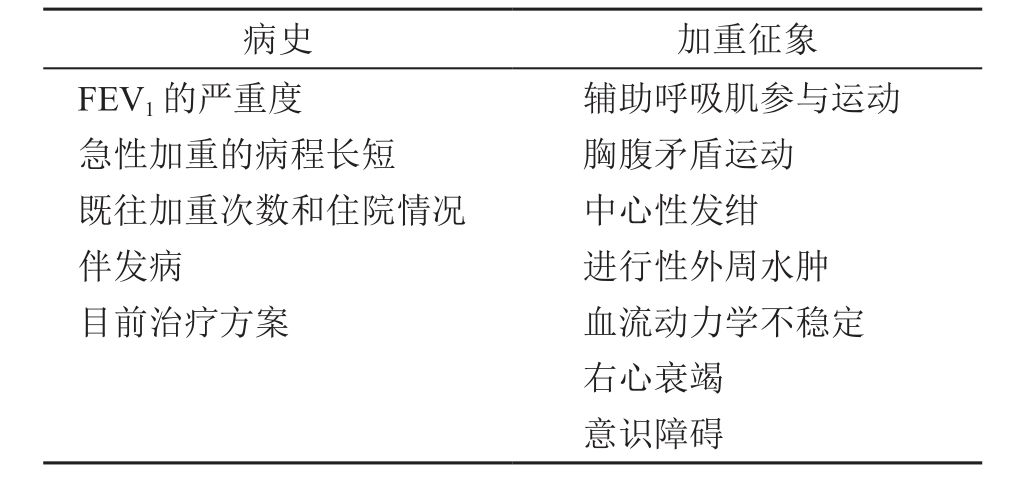
\includegraphics[width=3.35417in,height=1.58333in]{./images/Image00399.jpg}
\end{table}

低血压或高流量吸氧后动脉血氧分压(PaO\textsubscript{2}
)不能升至60mmHg以上提示有肺栓塞的可能。第一秒用力呼气容积(FEV\textsubscript{1}
)< 1L提示严重发作。PaO\textsubscript{2} <
50mmHg,动脉血二氧化碳分压(PaCO\textsubscript{2} )>70mmHg,pH <
7.30提示病情危重,需立即进行严密监护或收住重症监护病房(ICU)行无创或有创机械通气治疗

\subsubsection{实验室检查及其他监测指标}

\paragraph{肺活量和最大呼气流量}

肺功能检查是判断气流受限的客观指标,对COPD的诊断、严重程度评价、疾病进展、预后及治疗反应等均有重要意义。虽然肺功能检查操作简单,但加重期患者常难以满意地完成肺功能检查,并且在急性加重期这些测量结果往往不准确,故不作为常规推荐。此外,FEV\textsubscript{1}
< 1L可提示严重发作。

\paragraph{脉氧和动脉血气分析}

脉氧可用于评估患者的氧饱和度及实施氧疗的必要性,对于需住院治疗的患者,动脉血气分析是评估急性加重危险程度的重要指标。在吸入室内空气条件下PaO\textsubscript{2}
< 60mmHg和(或)SaO\textsubscript{2} <
90\%,伴或不伴PaCO\textsubscript{2} > 50mmHg提示呼吸衰竭。

\paragraph{胸部 X线检查和心电图}

胸部X线(后前位+侧位)有助于AECOPD与其他有类似症状的疾病相鉴别。ECG对心律失常、心肌缺血及右心室肥厚的诊断有帮助。螺旋CT、血管造影和血浆D-二聚体检测在诊断AECOPD患者发生肺栓塞时有重要作用,在此核素通气灌注扫描诊断价值不大。

\paragraph{其他实验室检查}

血红细胞计数及血细胞比容有助于了解有无红细胞增多症或出血。部分患者血白细胞计数增高及中性粒细胞核左移可为气道感染提供佐证。但通常白细胞计数并无明显改变。

\paragraph{痰培养及细菌药物敏感试验}

AECOPD有脓性痰者,应给予抗生素治疗,抗生素治疗前应进行痰培养及细菌药物敏感试验。若患者对初始抗生素治疗反应不佳时,应根据痰培养及细菌药物敏感试验结果进行调整。

\paragraph{血液生化检查}

有助于确定引起AECOPD的其他因素,如电解质紊乱(低钠、低钾和低氯血症等),糖尿病危象或营养不良等,也可发现合并存在的代谢性酸碱失衡。

\subsubsection{鉴别诊断}

部分AECOPD患者以突发意识障碍就诊,须与脑血管病、中毒等相鉴别。而以呼吸困难就诊,须与心力衰竭、气胸、胸腔积液以及急性肺血管栓塞症鉴别。

\subsection{治疗}

\subsubsection{确定COPD急性加重的原因}

引起COPD加重的最常见原因是气管-支气管感染,病原体主要是病毒、细菌。部分病例加重的原因难以确定,环境理化因素改变可能有作用。

\subsubsection{紧急处理}

急诊科应重视对COPD急性加重病情严重程度的紧急评估,具体方法为与患者加重前的病史、症状、体征、肺功能测定、动脉血气监测以及其他实验室检查指标进行比较,对判断AECOPD严重程度甚为重要。神志变化是COPD急性加重病情恶化及危重的标志,须紧急抢救。此外,辅助呼吸肌参与呼吸运动,胸腹矛盾呼吸、发绀、右心衰竭以及血流动力学不稳定均是急诊评估严重程度的独立指标。COPD急性加重常难以接受肺功能测定。动脉血气分析常提示呼吸衰竭(特征表现是PCO\textsubscript{2}
> 40mmHg伴或不伴PO\textsubscript{2} < 60mmHg),pH <
7.30提示病情严重。对经评估病情危重者需进行密切监护,必要时收住ICU行机械辅助通气等治疗。

\subsubsection{分层治疗策略}

\paragraph{居家治疗}

COPD急性加重早期病情较轻的患者可采取增加平素所使用的支气管舒张剂的剂量及给药频次治疗。未曾使用过抗胆碱药物者可选用异丙托溴铵或噻托溴铵吸入治疗,直至病情缓解;如未能缓解,可予较大剂量的雾化治疗,如沙丁胺醇2500μg加异丙托溴铵500μg,或沙丁胺醇1000μg加异丙托溴铵250~500μg雾化吸入,每日2~4次。全身使用糖皮质激素对加重期治疗有益,可促进病情缓解和肺功能恢复。如患者的基础FEV\textsubscript{1}
<
50\%预计值,除支气管舒张剂之外,可考虑口服糖皮质激素,泼尼松龙30~40mg,连用7~10天。或糖皮质激素联合长效β\textsubscript{2}
受体激动剂雾化吸入治疗。如患者咳痰量增多,痰液呈脓性,应积极给予抗生素治疗。抗生素选择应根据患者肺功能以及所处地区常见致病菌和耐药流行情况,选择敏感抗生素。主要病原微生物和具体用药见表\ref{tab98-2}。患者院外治疗期间需密切观察病情变化,以免贻误送医院治疗的时机。

\paragraph{住院治疗}

COPD急性加重病情严重者需住院治疗。AECOPD到医院急诊科就诊或住院治疗的指征:①症状显著加剧,如突然出现的静息状况下呼吸困难;②出现新的体征或原有体征加重(如发绀、外周水肿);③新近发生的心律失常;④有严重的伴随疾病;⑤初始治疗方案失败;⑥高龄COPD患者的急性加重;⑦诊断不明确;⑧院外治疗条件欠佳或治疗不力。AECOPD收入重症监护治疗病房(ICU)的指征:①严重呼吸困难且对初始治疗反应不佳;②精神障碍,嗜睡,昏迷;③经氧疗和无创性正压通气(NIPPV)后,低氧血症(PaO\textsubscript{2}
<
50mmHg)仍持续或呈进行性恶化,和(或)高碳酸血症(PaCO\textsubscript{2}
> 70mmHg)无缓解甚至有恶化,和(或)严重呼吸性酸中毒(pH <
7.30)无缓解,甚至恶化。

\subsubsection{AECOPD住院治疗方案}

1.根据症状 、血气、胸部X线片等评估病情的严重程度。

2.控制性氧疗
氧疗是COPD加重期住院患者的基础治疗。无严重并发症的COPD加重期患者氧疗后易达到满意的氧合水平(PaO\textsubscript{2}
> 60mmHg或SaO\textsubscript{2} >
90\%)。但吸入氧浓度不宜过高,需注意可能发生潜在的CO\textsubscript{2}
潴留及呼吸性酸中毒,给氧途径包括鼻导管或Venturi面罩,其中Venturi面罩更能精确地调节吸入氧浓度。氧疗30分钟后应复查动脉血气,以确认氧合满意,且未引起CO\textsubscript{2}
潴留及(或)呼吸性酸中毒。

\paragraph{支气管舒张剂治疗}

治疗AECOPD的支气管舒张剂首选β\textsubscript{2}
受体激动剂。如疗效不佳,推荐加用抗胆碱能药。对于较为严重的AECOPD,可考虑静脉滴注茶碱类药物。由于茶碱类药物血药浓度个体差异较大,治疗窗较窄,监测血清茶碱浓度对于评估疗效和避免不良反应都有一定意义。

\paragraph{糖皮质激素}

糖皮质激素在AECOPD中的疗效已被肯定,但治疗采用何种方案最适宜尚未达成共识。在AECOPD患者住院治疗期间,作为辅助治疗,推荐口服或静脉使用肾上腺皮质激素。由于大剂量使用肾上腺皮质激素与副作用风险增加相关,要权衡疗效及安全性。一般认为口服泼尼松龙30~40mg/d,7~10天安全有效。住院患者如果不能口服,可静脉给予甲泼尼龙40mg/d。在无酸中毒的AECOPD患者,亦可采用糖皮质激素(如布地奈德)雾化吸入替代口服治疗。激素联合长效β\textsubscript{2}
受体激动剂雾化吸入效果更好。延长疗程不会增加有效性,反而导致副作用(如高血糖、肌萎缩症等)风险增加。对特殊患者(合并糖尿病、高血压、消化性或应激性溃疡等)应用时需考虑到激素的不良反应,酌情减量或适时停药。

\paragraph{呼吸中枢兴奋剂治疗}

急性呼吸衰竭不推荐使用呼吸兴奋剂。静脉使用多沙普仑(doxapram),一种非特异性呼吸兴奋剂,相对安全,但仅推荐用于无法行无创通气治疗的患者。

\paragraph{抗生素}

\begin{table}[htbp]
\centering
\caption{AECOPD患者抗生素治疗参考表}
\label{tab98-2}
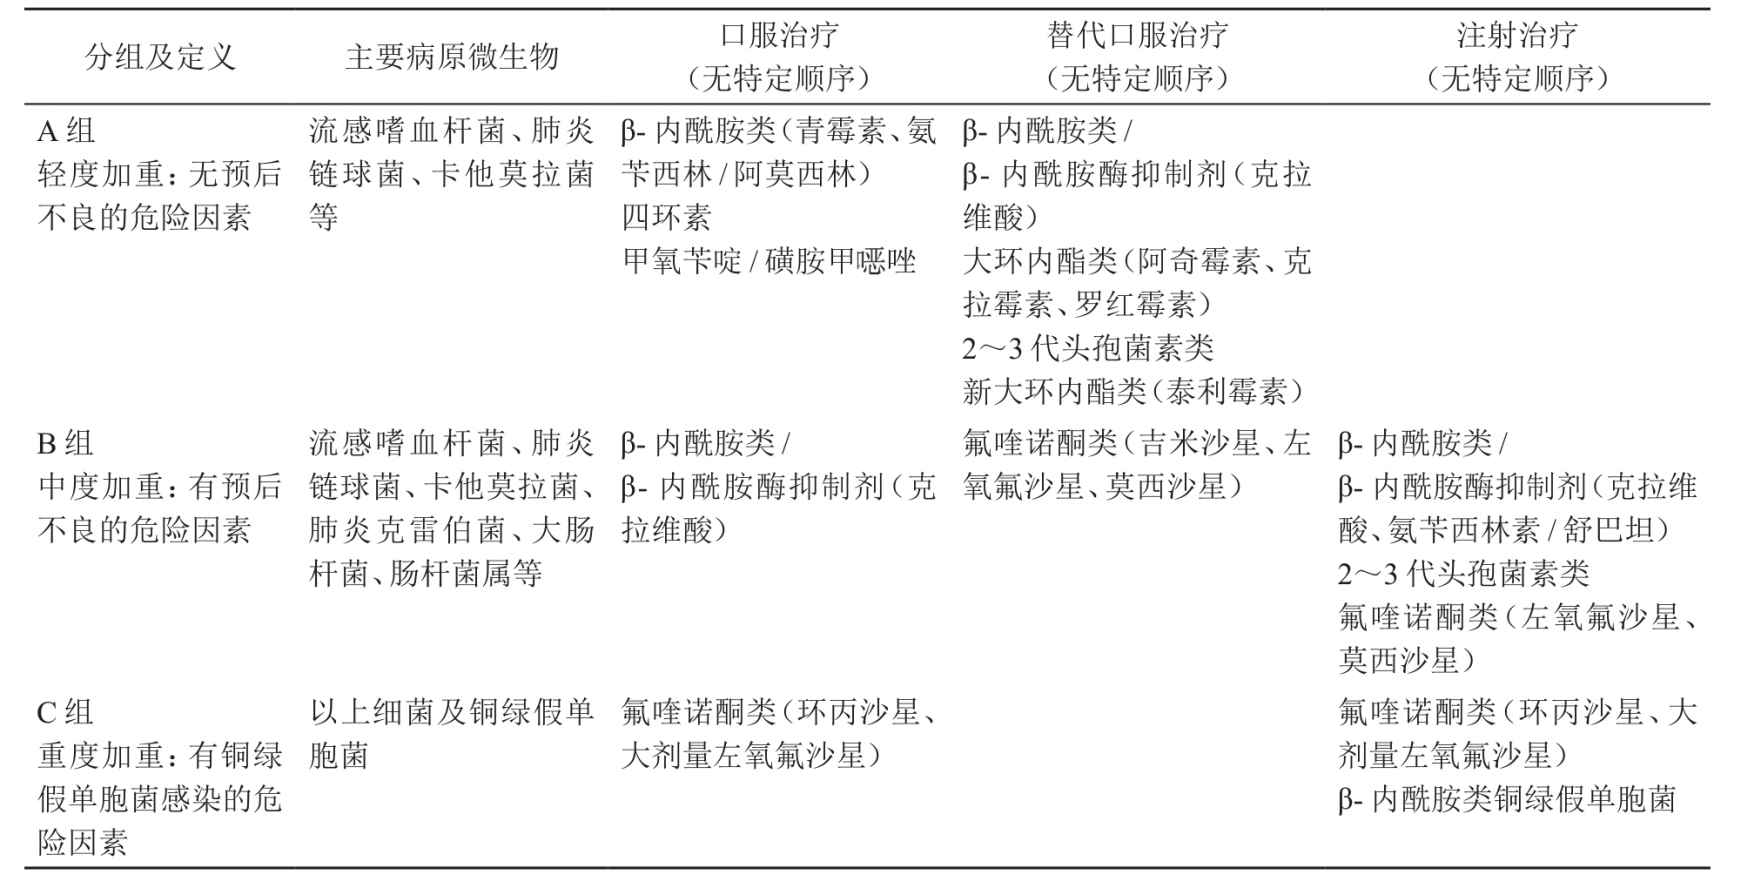
\includegraphics[width=6.73958in,height=3.39583in]{./images/Image00400.jpg}
\end{table}

COPD急性加重多由细菌感染诱发,故抗生素治疗在AECOPD治疗中具有重要地位。当患者呼吸困难加重,咳嗽伴有痰量增多及脓性痰时,应根据COPD严重程度及相应的细菌分层情况,结合当地区常见致病菌类型及耐药流行趋势和药物敏感情况尽早选择敏感抗生素。如对初始治疗方案反应欠佳,应及时根据细菌培养及药敏试验结果调整抗生素。随机对照研究证实,具有以下3项主征,即呼吸困难、痰量增多以及脓性痰的AECOPD患者可从抗生素治疗中获益;此外还发现需行无创或有创机械通气的AECOPD患者,如不使用抗生素治疗,死亡率及继发性医院获得性肺炎发生率显著升高,故推荐使用抗生素。通常COPD急性加重的感染源主要为病毒或细菌,其中主要致病菌多为肺炎链球菌、流感嗜血杆菌及卡他莫拉菌。除以上常见细菌外,尚可有肠杆菌科细菌、铜绿假单胞菌及耐甲氧西林金黄色葡萄球菌。发生铜绿假单胞菌的危险因素有:近期住院、频繁应用抗菌药物、以往有铜绿假单胞菌分离或寄植的历史等。要根据细菌可能的分布采用适当的抗菌药物治疗,主要病原微生物和具体用药参见表\ref{tab98-2}。总之,抗菌治疗应尽可能将细菌负荷降低到最低水平,以延长COPD急性加重的间隔时间。长期应用广谱抗生素和糖皮质激素易继发深部真菌感染,应密切观察真菌感染的临床征象并采用防治真菌感染措施。

\paragraph{机械通气}

机械通气可有无创或有创两种方式,根据病情需要,可首选无创性机械通气。无论是无创或有创机械通气都只是一种生命支持方式,在此支持条件下,通过药物治疗消除COPD加重的原因使急性呼吸衰竭得到逆转。进行机械通气的患者应有动脉血气监测。

\hypertarget{text00274.htmlux5cux23CHP9-6-3-4-5-1}{}
(1) 无创正压机械通气(noninvasive intermittent posive pressure
ventilation,NIPPV):

COPD急性加重期患者应用NIPPV可降低PaCO\textsubscript{2}
,减轻呼吸困难,从而降低气管插管和有创呼吸机的使用,缩短住院天数,降低患者病死率。使用NIPPV要注意掌握合理的操作方法,提高患者依从性,避免漏气,从低压力开始逐渐增加辅助吸气压和采用有利于降低PaCO\textsubscript{2}
的方法,从而提高NIPPV的效果。其应用适应证:①中~重度呼吸困难,辅助呼吸肌参与运动以及出现胸腹矛盾运动;②中~重度酸中毒(pH
< 7.35),和(或)高碳酸血症(PCO\textsubscript{2} >
45mmHg);③呼吸频率>
25次/分。相对禁忌证:①呼吸停止;②心血管系统功能不稳定(低血压、心律失常、心肌梗死);③精神异常,或不能配合;④存在高误吸风险;⑤气道大量分泌物;⑥近期面部或胃食管手术;⑦颅颌面外伤;⑧固有的鼻咽部异常;⑨烧伤;⑩极度肥胖。

\hypertarget{text00274.htmlux5cux23CHP9-6-3-4-5-2}{}
(2) 有创性机械通气:

在积极药物和NIPPV治疗后,患者呼吸衰竭仍进行性恶化,出现危及生命的酸碱失衡和(或)神志改变时宜用有创性机械通气治疗。病情好转后,根据情况可采用无创机械通气进行序贯治疗。有创性机械通气在COPD加重期的具体应用指征为:①对无创通气不能耐受或无创通气治疗失败;②严重呼吸困难,辅助呼吸肌参与运动以及出现胸腹矛盾运动;③呼吸频率>
35次/分;④威胁生命的低氧血症;⑤重度酸中毒(pH <
7.25),和(或)高碳酸血症(PCO\textsubscript{2} >
60mmHg);⑥呼吸停止;⑦严重心血管系统并发症(低血压、休克);⑧嗜睡,意识障碍;⑨其他并发症(代谢异常、脓毒症、肺炎、肺栓塞、气压伤、大量胸腔积液)。

目前使用最广泛的3种通气模式包括辅助控制通气(A-CMV),压力支持通气(PSV)或同步间歇强制通气(SIMV)与PSV联合模式(SIMV
+
PSV)。因COPD患者广泛存在内源性呼气末正压(PEEPi),为减少因PEEPi所致吸气功耗增加和人机不协调,可常规加用一适度水平(约为PEEPi的70\%~80\%)的外源性呼气末正压(PEEP)。COPD的撤机可能会遇到困难,需设计和实施周密方案。NIPPV已被用于帮助早期脱机并初步取得了良好的效果。

\paragraph{其他治疗措施}

监测出入量和血电解质,注意维持液体和电解质平衡;注意补充营养,对不能进食者需经胃肠补充要素饮食或予静脉高营养;对卧床、红细胞增多症或脱水的患者,无论是否有血栓栓塞性疾病史,均需考虑使用肝素或低分子肝素;积极排痰治疗(如刺激咳嗽,叩击胸部,体位引流等);及时识别并治疗伴随疾病(冠心病、糖尿病、高血压等)及并发症(休克、弥漫性血管内凝血、上消化道出血、胃功能不全等)。

\paragraph{出院和随访}

AECOPD患者出院标准:吸入β\textsubscript{2}
受体激动剂频率低于4小时1次,患者可在室内行走,可正常进食和睡眠(不被呼吸困难中断),症状稳定达12~24小时,血气稳定达12~24小时,患者(家属)充分理解并配合医嘱,完成随访以及居家照护事宜安排,患者、家属和医师均确定患者病情适合居家治疗和巩固疗效。

\protect\hypertarget{text00275.html}{}{}

\hypertarget{text00275.htmlux5cux23CHP9-6-4}{}
参 考 文 献

1.
中华医学会呼吸病学分会慢性阻塞性肺疾病学组.慢性阻塞性肺疾病诊治指南(2007年修订版).中华结核和呼吸杂志,2007,30(1):8-17

2. Gunen H,Hacievliyagil SS,Kosar F,et al. Factors affecting survival
of hospitalized patients with COPD. Eur Respir J,2005,26(2):234-241

3. Herber P,Tashkin DP,Simmons M,et al. Effect of occupational
exposures on decline of lung function in early chronic obstructive
pulmonary diseases. Am J Respir Crit Care
Med,2007,175(10):994-1000.

4. Sethi S,Evans N,Grant BJ,et al. New strain of bacteria and
exacerbations of chronic obstructive pulmonary disease. N Engl J
Med,2002,347(7):465-471.

5. Quon BS,Gan WQ,Sin DD. Contemporary management of acute
exacerbations of COPD:a systematic review and metaanalysis.
Chest,2008,133(3):756-766.

6. Rodríguez-Roisin R. COPD exacerbations.5:management.
Thorax,2006,61(6):535-544.

7. Ram FS,Rodriguez RR,Granados NA,et al. Antibiotics for
exacerbations of chronic obstructive pulmonary disease. Cochrane
Database Syst Rev,2006,19(2):CD004403.

8.
慢性阻塞性肺疾病无创机械通气治疗研究协作组.早期应用无创正压通气治疗慢性阻塞性肺疾病急性加重期患者的多中心随机对照研究.中华结核和呼吸杂志,2005,28
(10):680-684

\protect\hypertarget{text00276.html}{}{}

\chapter{肺 脓 肿}

肺脓肿(lung
abscess)是肺组织坏死形成的脓腔。临床特征为高热、咳嗽和咳大量脓臭痰。胸部X线显示一个或多个的含气液平的空洞,如多个直径小于2cm的空洞则称为坏死性肺炎。多发生于壮年,男多于女。自抗生素广泛使用以来,本病的发生率已明显降低。

\subsection{病因与发病机制}

急性肺脓肿的感染细菌常为上呼吸道、口腔的定植菌。包括需氧、厌氧和兼性厌氧菌。90\%的患者合并有厌氧菌感染,毒力较强的厌氧菌在部分患者可单独致病。常见的其他病原体包括金黄色葡萄球菌(金葡菌)、化脓性链球菌、肺炎克雷伯杆菌和铜绿假单胞菌。大肠埃希菌和流感嗜血杆菌也可引起坏死性肺炎。根据感染途径,肺脓肿可分为以下类型:

\paragraph{吸入性肺脓肿}

病原体经口、鼻、咽腔吸入致病,为肺脓肿发病的最主要原因。正常情况下,吸入物(如口腔、鼻、咽部手术后的血块;齿垢或呕吐物等)经气道黏液-纤毛运载系统、咳嗽反射和肺巨噬细胞可迅速清除。但当有意识障碍如在全身麻醉、酒醉、药物过量、癫痫、脑卒中时,或由于受寒、过度疲劳、全身免疫力与气道防御清除功能降低,吸入的病原菌可致病。此外,还可由于扁桃体炎、鼻窦炎、齿槽脓溢或龋齿等脓性分泌物被吸入致病。本型常为单发性,其发生与支气管解剖及体位有关。由于右总支气管较陡直,且管径较粗,吸入性分泌物易吸入右肺,故右肺发病多于左肺。在仰卧时,好发于上叶后段或下叶背段,在坐位时,好发于下叶后基底段。右侧位时,好发于右上叶前段和后段形成的腋亚段。病原体多为厌氧菌。

\paragraph{血源性肺脓肿}

皮肤创伤感染、疖痈、骨髓炎、中耳炎、产后盆腔感染等所致的菌血症,菌栓经血道播散到肺,引起小血管栓塞、炎症和坏死而形成肺脓肿。静脉吸毒者如有右心细菌性心内膜炎,三尖瓣赘生物脱落阻塞肺小血管形成肺脓肿,常为双肺外野的多发性脓肿。病原菌以金葡菌、表皮葡萄球菌及链球菌常见。

\paragraph{继发性肺脓肿}

在肺部其他疾病基础上,如某些细菌性肺炎(金葡菌、铜绿假单胞菌和肺炎克雷伯杆菌等)、支气管扩张、支气管囊肿、空洞性肺结核等产生继发感染而发病。支气管肺癌或误吸异物阻塞支气管,诱发引流支气管远端肺组织感染而形成肺脓肿。支气管异物阻塞是小儿肺脓肿的重要因素。亦有肺癌本身迅速增长,以致血供不足,发生中央性坏死伴发感染形成脓肿。肺部邻近器官感染病变如膈下脓肿、阿米巴肝脓肿扩散蔓延穿破膈肌进入肺部,引起肺脓肿。此外,肾周围脓肿、脊柱旁脓肿、食管穿孔等,穿破至肺亦可形成脓肿。

如急性肺脓肿治疗不彻底,或支气管引流不畅,导致大量坏死组织残留脓腔,炎症迁延3个月以上则称为慢性肺脓肿。

\subsection{诊断}

\subsubsection{临床表现特点}

吸入性肺脓肿患者多有齿、口、咽喉的感染灶,或上述降低呼吸道局部、全身抵抗力的诱因。起病急骤,患者畏寒、发热,体温多呈弛张热或(和)稽留热,达39~40℃,全身关节及肌肉酸痛,乏力,胃纳差。伴咳嗽,随感染加重,痰量则逐渐增加。从干咳转为咳黏液痰或黏液脓痰。如感染不能及时控制,于发病后10~14天,咳嗽加剧,脓肿溃破入支气管,突然有大量脓痰及脓肿坏死组织咳出,痰量每日可达300~500ml。约1/3患者伴有不同程度的咯血,偶有中、大量咯血而突然窒息致死。伴随大量脓痰的咳出,全身中毒症状明显减轻,热度迅速下降。腐臭脓痰提示厌氧菌感染,但无臭痰液亦不能排除厌氧菌,因为如微嗜氧和厌氧链球菌感染并不产生腐臭痰。典型肺脓肿痰静置后可分三层,上层为黏液及泡沫,中层为浆液,下层为脓块及坏死组织。如炎症波及局部胸膜可引起胸痛;病变范围较大,可出现气急。肺脓肿破溃到胸膜腔,可出现突发性胸痛、气急,出现脓气胸。部分患者缓慢发病,仅有一般的呼吸道感染症状。血源性肺脓肿多先有原发病灶引起的畏寒、高热等全身脓毒血症的症状,经数日至两周才出现肺部症状,如咳嗽、咳痰等,通常痰量不多,极少咯血。慢性肺脓肿患者有慢性咳嗽、咳脓痰、反复咯血、继发感染和不规则发热等,常呈贫血、消瘦、慢性消耗病态。肺脓肿的体征与肺脓肿的大小和部位有关,病变较小或位于肺脏的深部,可无异常体征;病变较长,脓肿周围有大量炎症,叩诊呈浊音或实音,听诊呼吸音减低,有时可闻湿啰音;血源性肺脓肿体征常阴性;慢性者有杵状指(趾)。

\subsubsection{辅助检查}

\paragraph{血象}

白细胞计数可达20 × 10\textsuperscript{9} /L以上,中性粒细胞比值>
0.8~0.9,核明显左移,常有中毒颗粒。慢性者血细胞无明显改变,但可有轻度贫血。

\paragraph{病原学检查}

痰液涂片革兰染色检查,痰、胸腔积液和血培养,包括厌氧菌培养和药敏试验,有助于确定病原菌和选择有效的抗生素。尤其是胸腔积液和血培养阳性时对致病菌的诊断价值更大。

\paragraph{X线检查}

肺脓肿的X线表现根据类型、病期、支气管的引流是否通畅以及有无胸膜并发症而有所不同。吸入性肺脓肿在早期化脓性炎症阶段,其典型的X线征象为大片浓密模糊炎性浸润阴影,边缘不清,分布在一个或数个肺段,与细菌性肺炎相似。脓肿形成后,大片浓密炎性阴影中出现圆形透亮区及液平面。在消散期,脓腔周围炎症逐渐吸收,脓腔缩小而至消失,最后残留少许纤维条索阴影。慢性肺脓肿脓腔壁增厚,内壁不规则,周围炎症略消散,但不完全,伴纤维组织显著增生,并有程度不等的肺叶收缩,胸膜增厚。纵隔向患侧移位,其他健肺发生代偿性肺气肿。血源性肺脓肿在一侧肺或双肺边缘部有多发的散在小片状炎症阴影或边缘较整齐的球形病灶,其中可见脓腔及液平面。炎症吸收后可呈现局灶性纤维化或小气囊。并发脓胸者,患侧胸部呈大片浓密阴影;若伴发气胸则可见液平面。侧位X线检查,可明确脓肿在肺脏中的部位及其范围大小。

\paragraph{CT检查}

CT能更准确定位及区别肺脓肿和有气液平的局限性脓胸、发现体积较小的脓肿和葡萄球菌肺炎引起的肺气囊,并有助于作体位引流或外科治疗。

\paragraph{纤维支气管镜检查}

应列为常规,可达诊断和治疗双重目的。若为支气管肿瘤,可摘取作活检,考虑外科根治手术;还可取痰液标本行病原学检查。如见到异物可摘(取)出,使引流恢复通畅。亦可借助纤维支气管镜吸引脓液和病变部注入抗生素,促进支气管引流和脓腔的愈合,以提高疗效与缩短病程。

\subsubsection{诊断注意事项}

对有口腔手术、昏迷呕吐、异物吸入后,突发畏寒、高热、咳嗽和咳大量脓臭痰等病史的患者,其血白细胞总数及中性粒细胞显著增高,结合胸部X线表现,可作出诊断。有皮肤创伤感染、疖、痈等化脓性病灶,或静脉吸毒者患心内膜炎,出现发热不退并有咳嗽、咳痰等症状,胸部X线检查示有两肺多发性小脓肿,可诊断为血源性肺脓肿。血、痰培养,包括厌氧菌培养及药敏试验,对确定病因诊断和抗菌药物的选用有重要价值。肺脓肿应注意与以下疾病相鉴别:

\paragraph{细菌性肺炎}

早期肺脓肿与细菌性肺炎在症状及X线表现上很相似。细菌性肺炎中肺炎链球菌肺炎最常见,常有口唇疱疹、铁锈色痰而无大量脓臭痰;X线胸片示肺叶或肺段实变,或呈片状淡薄性病变,边缘模糊不清,但无脓腔形成。其他有化脓性倾向的葡萄球菌、肺炎克雷伯杆菌肺炎等,痰或血的细菌培养与分离可作出鉴别。当用抗菌药物治疗后仍高热不退、咳嗽、咳痰加剧并咳出大量脓臭痰时应考虑为肺脓肿。

\paragraph{支气管肺癌}

支气管肺癌阻塞支气管常引起远端肺化脓性感染而形成肺脓肿。但其形成肺脓肿的病程相对较长,有一个逐渐阻塞的过程,中毒症状不明显,脓痰量亦较少。阻塞性感染多由于支气管引流不畅,抗菌药物疗效不佳。因此,对40岁以上出现同一部位反复肺部感染,且抗生素治疗效果不满意的患者,应考虑支气管肺癌引起阻塞性肺炎的可能,可送痰液找癌细胞和做纤维支气管镜检查,以明确诊断。肺鳞癌本身亦可发生坏死液化形成癌性空洞,但无急性起病和明显中毒症状,临床多有刺激性咳嗽和咯血,胸部X线片示空洞常呈偏心、壁较厚、内壁凹凸不平,一般无液平面,空洞周围无炎症反应,外壁呈分叶状,有脐样切迹或细小毛刺。由于癌肿经常发生转移,故常见到肺门淋巴结肿大。纤维支气管镜和痰脱落细胞学检查可明确诊断。

\paragraph{空洞性肺结核继发感染}

发病缓慢,病程长,常伴有结核毒性症状,如午后低热、乏力、盗汗、长期咳嗽、咯血等。病灶多位于肺上部。胸部X线片示空洞壁较厚,其周围可见结核浸润病灶,或伴有斑点、结节状病变,空洞内一般无液平面,有时伴有同侧或对侧的结核播散病灶。痰中可找到结核杆菌。但是一旦并发细菌化脓性感染时,急性感染症状和体征就会非常突出,阳性结核杆菌也可以因化脓性感染细菌的大量繁殖而难以检出,因此,没有过去典型结核病病史或临床表现的病例,极易将结核性空洞继发感染误诊为肺脓肿。如一时不能鉴别,按急性肺脓肿治疗控制急性感染后,胸片即可显示纤维空洞及周围结核病变,痰结核杆菌也可能阳转。

\paragraph{肺囊肿继发感染}

继发感染时,囊肿内可见气液平,周围炎症反应轻,无明显中毒症状和脓痰。而且随感染的控制,炎症消散,囊肿壁薄、光洁整齐为其特征。若有感染前的X线片相比较,则更易鉴别。

\subsection{治疗}

肺脓肿的治疗原则是抗菌药物治疗和脓液引流。

\subsubsection{抗菌药物治疗}

急性吸入性肺脓肿多为厌氧菌感染,一般都对青霉素敏感,青霉素常为首选药物。仅脆弱拟杆菌对青霉素不敏感,但对林可霉素(洁霉素,lincomycin)、克林霉素(氯洁霉素,clindamycin)和甲硝唑(metronidazole)敏感。青霉素剂量根据病情,轻症120万~240万U/d,严重者1000万U/d分次静脉滴注。在有效抗生素治疗下,体温约3~10天可下降至正常。此时可将静脉给药转换为肌注。若青霉素疗效不佳,可用林可霉素1.8~3.0g/d分次静脉滴注,或克林霉素0.6~1.8g/d,或甲硝唑0.4g,每日3次口服或静滴。血源性肺脓肿多为葡萄球菌和链球菌感染,可选用耐β-内酰胺酶的青霉素类或头孢菌素,对MRSA则需用万古霉素或替考拉宁。如为阿米巴原虫感染,则用甲硝唑治疗。如为革兰阴性杆菌,则可选用第二、三代头孢菌素、氟喹诺酮类,可联用氨基糖苷类抗生素。如庆大霉素(16万~24
万U/d)、阿米卡星(丁胺卡那霉素,0.4~0.6g/d)、妥布霉素(160~240mg/d)等。有条件时最好参考细菌培养和药敏试验结果调整和选择抗生素。

抗生素疗程一般为8~12周左右,或直至临床症状完全消失,X线片显示脓腔及炎性病变完全消散,仅残留条索状纤维阴影为止。

\subsubsection{脓液引流}

祛痰药如氯化铵0.3g,鲜竹沥10~15ml,每日3次口服,可使痰液易咳出。痰浓稠者,可用气道湿化如蒸汽吸入,超声雾化吸入等以利痰液的引流。体位引流排脓是缩短病程、加速病灶愈合、提高治愈率的重要环节,对一般情况好、发热不高的患者,使脓肿部位处于高位,在患部轻拍,每日2~3次,每次10~15分钟。但对脓液甚多且身体虚弱者体位引流应慎重,以免大量脓痰涌出,不及时咳出而造成窒息。有明显痰液阻塞征象,可经纤维支气管镜冲洗并吸引。贴近胸壁的巨大脓腔,可留置导管引流和冲洗。合并脓胸时应尽早胸腔抽液、引流。

\subsubsection{外科手术治疗}

适应证有:①肺脓肿病程超过3个月,经内科治疗脓腔不缩小,或脓腔过大(>
5cm)估计不易闭合者;②大咯血经内科治疗无效或危及生命;③伴有支气管胸膜瘘或脓胸经抽吸、引流和冲洗疗效不佳者;④支气管阻塞疑为支气管肺癌者。

\protect\hypertarget{text00277.html}{}{}

\hypertarget{text00277.htmlux5cux23CHP9-7-4}{}
参 考 文 献

1. 郝利明 .吸入性肺脓肿51例临床回顾.中国实用内科杂志,1994,14(1):39

2. 陆再英,钟南山.内科学.第7版.北京:人民卫生出版社,2008:35

\protect\hypertarget{text00278.html}{}{}

\chapter{肺 栓 塞}

肺栓塞(pulmonary
embolism,PE)是内源性或外源性栓子堵塞肺动脉或其分支所致肺循环障碍的一组临床和病理生理综合征,包括肺血栓栓塞症(pulmonary
thromboembolism,PTE)、脂肪栓塞综合征、羊水栓塞、空气栓塞、肿瘤栓塞等。来自静脉系统或右心的血栓堵塞肺动脉或其分支引起的肺循环和呼吸功能障碍的临床和病理综合征称为PTE,临床上95\%以上的PE是由于PTE所致,是最常见的PE类型,因此,临床上所说的PE通常指的是PTE。PE中80\%~90\%的栓子来源于下肢深静脉血栓,临床上又把PE和深静脉血栓形成(deep
venous thrombosis,DVT)划归于静脉血栓栓塞症(venous
thromboembolism,VTE),并认为PE和DVT具有相同的易患因素,大多数情况下二者伴随发生,为VTE的两种不同临床表现形式。PE可单发或多发,但常发生于右肺和下叶。当栓子堵塞肺动脉,如果其支配区的肺组织因血流受阻或中断而发生坏死,称之为肺梗死(pulmonary
infarction,PI)。由于肺组织同时接受肺动脉、支气管动脉和肺泡内气体三重供氧,因此肺动脉阻塞时临床较少发生肺梗死。如存在基础心肺疾病或病情严重,影响到肺组织的多重氧供,才有可能导致PI。

经济舱综合征(economy class
syndrome,ECS)是指由于长时间空中飞行,静坐在狭窄而活动受限的空间内,双下肢静脉回流减慢,血液淤滞,从而发生DVT和(或)PTE,又称为机舱性血栓形成。长时间坐车(火车、汽车、马车等)旅行也可以引起DVT和(或)PTE,故广义的ECS又称为旅行者血栓形成(traveler's
thrombosis)。

“e栓塞”:是指上网时间比较长而导致的下肢静脉血栓形成并栓塞的事件,与现代工作中电脑普及以及相应工作习惯有关。

\subsection{病因与发病机制}

PE的栓子99\%是属血栓性质的,因此,导致血栓形成的危险因素均为PE的病因。这些危险因素包括原发性及获得性危险因素,原发性危险因素一般指的是血液中一些抗凝物质及纤溶物质先天性缺损,如凝血酶原20210A基因突变、蛋白C缺乏、蛋白S缺乏、抗凝血酶Ⅲ(ATⅢ)缺乏等,常以反复静脉血栓形成和栓塞为主要临床表现。若40岁以下的年轻患者无明显诱因反复发生DVT和PTE,或发病呈家族聚集倾向,应注意做相关原发性危险因素的检查。获得性危险因素临床常见有:高龄、长期卧床、长时间旅行、动脉疾病(含颈动脉及冠状动脉病变)、近期手术史、创伤或活动受限如卒中、肥胖、真性红细胞增多症、管状石膏固定患肢、VTE病史、急性感染、抗磷脂抗体综合征、恶性肿瘤、妊娠、口服避孕药或激素替代治疗等。另外随着医学科学技术的发展,心导管、有创性检查及治疗技术(如ICD植入和中心静脉置管等)的广泛开展,也大大增加了DVT-PE的发生,因此充分重视上述危险因素将有助于对PE的早期识别。

引起PTE的血栓可以来源于下腔静脉径路、上腔静脉径路或右心腔,其中大部分来源于下肢深静脉,尤其是从腘静脉上端到髂静脉段的下肢近端深静脉(约占50\%~90\%)。盆腔静脉丛亦是血栓的重要来源。

由于PE致栓塞部位肺血流量减少,机械性肺毛细血管前动脉高压,加之肺动脉、冠状动脉反射性痉挛,使肺毛细血管床减少,肺循环阻力增加,肺动脉压力上升,使右心负荷加重,心排血量下降。又由于右心负荷加重致右心压力升高,右室扩张致室间隔左移,导致左室舒张末期容积减少和充盈减少,使主动脉与右室压力阶差缩小及左心室功能下降,进而心排血量减少,体循环血压下降,冠状动脉供血减少及心肌缺血,致脑动脉及冠状动脉供血不足,患者可发生脑供血不足、脑梗死、心绞痛、急性冠状动脉综合征、心功能不全等。肺动脉压力升高程度与血管阻塞程度有关。由于肺血管床具备强大的储备能力,对于原无心肺异常的患者,肺血管床面积减少25\%~30\%时,肺动脉平均压轻度升高;肺血管床面积减少30\%~40\%时,肺动脉平均压可达30mmHg以上,右室平均压可升高;肺血管床面积减少40\%~50\%时,肺动脉平均压可达40mmHg,右室充盈压升高,心排血指数下降;肺血管床面积减少50\%~70\%时,可出现持续性肺动脉高压;肺血管床面积减少达85\%以上时,则可发生猝死。既往患有心肺疾患的患者出现上述情况时,肺动脉压力变化则更为明显。较小的和远端的栓子虽不影响血流动力学,但可使肺泡出血致咯血、胸膜炎和轻度的胸膜渗出,临床表现为“肺梗塞”。PE后堵塞部位肺仍保持通气,但无血流,肺泡不可充分地进行气体交换,致肺泡无效腔增大,导致肺通气血流比例失调,低氧血症发生。PE时由于低氧血症及肺血管内皮功能损伤,释放内皮素、血管紧张素Ⅱ,加之血栓中的血小板活化脱颗粒释放5-羟色胺、缓激肽、血栓素A、二磷酸腺苷、血小板活化因子等大量血管活性物质,均进一步使肺动脉血管收缩,致肺动脉高压等病理生理改变。

若急性PE后肺动脉内血栓未完全溶解,或反复发生PTE,则可能形成慢性血栓栓塞性肺动脉高压(CTEPH),继而出现慢性肺心病,右心代偿性肥厚和右心衰竭。

\subsection{诊断}

\subsubsection{临床表现特点}

PE发生后临床表现多种多样,可涉及呼吸、循环及神经系统等多个系统,但是缺乏特异性。其表现主要取决于栓子的大小、数量、与肺动脉堵塞的部位、程度、范围,也取决于过去有无心肺疾患、血流动力学状态、基础心肺功能状态、患者的年龄及全身健康状况等。较小栓子可能无任何临床症状。小范围的PE(面积小于肺循环50\%的PE)一般没有症状或仅有气促,以活动后尤为明显。当肺循环>
50\%突然发生栓塞时,就会出现严重的呼吸功能和心功能障碍。

\paragraph{症状}

常见症状有:①不明原因的呼吸困难及气促,尤以活动后明显,为PE最重要、最常见症状,发生率为80\%~90\%。②胸痛:为PE常见的症状,发生率为40\%~70\%,可分为胸膜炎性胸痛(40\%~70\%)及心绞痛样胸痛(4\%~12\%)。胸膜炎性胸痛常为较小栓子栓塞周边的肺小动脉,局部肺组织中的血管活性物质及炎性介质释放累及胸膜所致。胸痛多与呼吸有关,吸气时加重,并随炎症反应消退或胸腔积液量的增加而消失。心绞痛样胸痛常为较大栓子栓塞大的肺动脉所致,是梗死面积较大致血流动力学变化,引起冠状动脉血流减少,患者发生典型心绞痛样发作,发生时问较早,往往在栓塞后迅速出现。③晕厥:发生率为11\%~20\%,为大面积PE所致心排血量降低致脑缺血,值得重视的是临床上晕厥可见于PE首发或唯一临床症状。出现晕厥往往提示预后不良,有晕厥症状的PTE死亡率高达40\%,其中部分患者可猝死。④咯血:约占10\%~30\%,多于梗死后24小时内发生,常为少量咯血,大咯血少见,多示肺梗死发生。⑤烦躁不安、惊恐甚至濒死感:多示梗死面积较大,与严重呼吸困难或胸痛有关。⑥咳嗽、心悸等。各病例可出现以上症状的不同组合。临床上有时出现所谓“三联征”,即同时出现呼吸困难、胸痛及咯血,但仅见于20\%的患者。

\paragraph{体征}

常见体征有:①呼吸系统:呼吸急促最常见;发绀;肺部有时可闻及哮鸣音和(或)细湿啰音;合并肺不张和胸腔积液时出现相应的体征。②循环系统:心动过速,主要表现为窦性心动过速,也可发生房性心动过速、心房纤颤、心房扑动或室性心律失常;多数患者血压可无明显变化,大面积PE可有血压下降,甚至休克;颈静脉充盈、怒张,或搏动增强;肺动脉瓣区第二心音亢进或分裂,三尖瓣可闻收缩期杂音。③其他:可伴发热,多为低热。

\paragraph{DVT的症状与体征}

下肢DVT的主要表现为患肢肿胀、周径增粗、疼痛或压痛、皮肤色素沉着,行走后患肢易疲劳或肿胀加重。但半数以上的下肢DVT患者无自觉症状和明显体征。应测量双侧下肢的周径来评价其差别,大、小腿周径的测量点分别为髌骨上缘以上15cm处,髌骨下缘以下10cm处。双侧相差>
1cm即考虑有临床意义。

\subsubsection{辅助检查}

\paragraph{胸部 X线检查}

PE时X线检查可有以下征象:①肺动脉阻塞征:区域性肺血管纹理纤细、稀疏或消失,肺野透亮度增加;②肺动脉高压征及右心扩大征:右下肺动脉干增宽或伴截断征,肺动脉段膨隆以及右心室扩大;③肺组织继发改变:肺野局部片段阴影,尖端指向肺门的楔形阴影,肺不张或膨胀不全,肺不张侧可见膈肌抬高,有时合并胸腔积液。

\paragraph{心电图}

心电图改变是非特异性的,常是一过性的、多变的,需动态比较观察有助于诊断。常见的心电图改变是电轴右偏;S\textsubscript{Ⅰ}
Q\textsubscript{Ⅲ} T\textsubscript{Ⅲ} (Ⅰ导联S波变深,S波>
1.5mm,Ⅲ导联有Q波和T波倒置);右心前导联及Ⅱ、Ⅲ、aVF导联T波倒置;完全性或不完全性右束支传导阻滞等。应与非ST段抬高性急性冠脉综合征进行鉴别。

\paragraph{动脉血气分析}

尽管血气分析的检测指标不具有特异性,但有助于对PE的筛选。为提高血气分析对PE诊断的准确率,应以患者就诊时卧位、未吸氧、首次动脉血气分析的测量值为准。由于动脉血氧分压随年龄的增长而下降,所以血氧分压的正常预计值应按照公式PaO\textsubscript{2}
(mmHg)= 106 − 0.14
×年龄(岁)进行计算。70\%~86\%的患者示低氧血症及呼吸性碱中毒,93\%的患者有低碳酸血症,86\%~95\%的患者肺泡-动脉血氧分压差P(A-a)O\textsubscript{2}
增加(> 15mmHg)。

\paragraph{超声心动图}

在提示诊断和除外其他心血管疾患方面有重要价值。对于严重的PTE病例,可以发现右室壁局部运动幅度降低;右室和(或)右房扩大;室间隔左移和运动异常;近端肺动脉扩张;三尖瓣反流速度增快;下腔静脉扩张,吸气时不萎陷。若在右房或右室发现血栓,同时患者临床表现符合PTE,可作出诊断。偶可因发现肺动脉近端的血栓而直接确诊。

\paragraph{放射性核素肺通气灌注扫描}

本项检查是二线诊断手段,通常禁用于肾功能不全、造影剂过敏或者孕妇。严重肺动脉高压,中度以上心脏内右向左分流及肺内分流者禁用此诊断方法。典型征象是与通气显像不匹配的肺段分布灌注缺损。其诊断肺栓塞的敏感性为92\%,特异性为87\%,且不受肺动脉直径的影响,尤其在诊断亚段以下肺动脉血栓栓塞中具有特殊意义。但下述情况也可致肺灌注显像呈假阳性改变,故需排除:血管腔外受压(肿瘤、气胸、胸腔积液)、支气管扩张及慢性肺部炎症、慢性阻塞性肺疾患、左心衰竭、肺囊肿、陈旧性肺结核、肺切除术后。为提高诊断正确率,减少假阳性率,可同时作双下肢静脉显像,与胸部X线平片、CT肺动脉造影相结合,可大大提高诊断率。

\paragraph{多层螺旋 CT肺动脉造影}

目前已广泛用于临床,是PE的主要确诊手段之一。可显示主肺动脉、左右肺动脉及其分支的血栓或栓子,不仅能够发现段以上肺动脉内的栓子,对亚段PE的诊断价值较高。PE的直接征象为肺动脉内的低密度充盈缺损,部分或完全包围在不透光的血流之间(轨道征),或者呈完全充盈缺损,远端血管不显影。间接征象包括肺野楔形密度增高影,条带状的高密度区或盘状肺不张,中心肺动脉扩张及远端血管分支减少或消失等右心室改变的征象。

\paragraph{肺动脉造影}

是公认诊断PE的金指标,属有创性检查,不作为PTE诊断的常规检查方法。肺动脉造影可显示直径1.5mm的血管栓塞,其敏感性为98\%,特异性为95\%~98\%。肺动脉造影影像特点为:直接征象为血管腔内造影剂充盈缺损,伴或不伴轨道征的血流阻断;间接征象为栓塞区域血流减少及肺动脉分支充盈及排空延迟。多在患者需要介入治疗如导管抽吸栓子、直接肺动脉内溶栓时应用。

\paragraph{下肢深静脉检查}

对于PE来讲这项检查十分重要,可寻找PE栓子的来源,资料显示PE的栓子80\%~90\%来源于下肢深静脉血栓形成,对于存在下肢深静脉血栓(DVT)者近半数患者可发生PE,尤其对双下肢不对称肿胀者,在同一水平的周径相差>
1.0cm的患者,必须作此项检查。

\hypertarget{text00278.htmlux5cux23CHP9-8-2-2-8-1}{}
(1) 血管超声多普勒检查:

为首选方法,可对血管腔大小、管壁厚度及管腔内异常回声均可直接显示,其诊断准确率为88\%~93\%。

\hypertarget{text00278.htmlux5cux23CHP9-8-2-2-8-2}{}
(2) CT肺血管造影(CTPA)加CT静脉造影:

此方法为目前临床常用的方法,可对PE及DVT作为统一整体检查,可于静脉期对腹腔、盆腔和下肢静脉采像,检测DVT,其准确性优于超声检查。

\paragraph{血浆}

D-二聚体测定
为目前诊断PE及DVT的常规实验室检查方法。由于血浆中2\%~3\%的血浆纤维蛋白原转变为血浆蛋白,故正常人血浆中可检测到微量D-二聚体,如>
500μg/L对诊断PE有指导意义,若<
500μg/L有重要的排除诊断价值。D-二聚体水平与血栓大小、堵塞范围无明显关系。D-二聚体测定敏感性高而特异性差,外科手术、外伤和急性心肌梗死时D-二聚体也可增高。本项检查尤适合于急诊室怀疑PE同时不合并其他急性系统性疾病的患者。

\subsubsection{诊断注意事项}

\hypertarget{text00278.htmlux5cux23CHP9-8-2-3-1}{}
(一) PE的诊断程序

PE的临床表现多样,有时隐匿,缺乏特异性,确诊需特殊检查。检出PE的关键是提高诊断意识。PE诊断程序一般包括疑诊、确诊、求因三个步骤:

\paragraph{根据临床情况疑诊 PE(疑诊)}

如患者出现上述临床表现特点,尤其是在存在危险因素(包括任何可以导致静脉血液淤滞、静脉系统内皮损伤和血液高凝状态的因素)的病例出现不明原因的呼吸困难、胸痛、晕厥、休克,或伴有单侧或双侧不对称性下肢肿胀、疼痛等,应进行如下检查:①血浆D-二聚体(D-dimer)测定;②动脉血气分析:③心电图;④X线胸片;⑤超声心动图;⑥下肢深静脉超声检查。

\paragraph{对疑诊病例进一步明确诊断(确诊)}

在临床表现和初步检查提示PE的情况下,应安排PE的确诊检查,包括以下4项,其中1项阳性即可明确诊断:①螺旋CT肺动脉造影(CTPA);②放射性核素肺通气/血流灌注扫描;③磁共振显像(MRI);④肺动脉造影。

\paragraph{寻找 PE的成因和危险因素(求因)}

对某一病例只要疑诊PE,无论其是否有DVT症状,均应进行体检,并行下肢深静脉检查(包括下肢深静脉血管超声多普勒检查、放射性核素下肢深静脉造影、CT静脉造影、MRI静脉造影、肢体阻抗容积图等),以帮助明确是否存在DVT及栓子的来源。同时要注意患者有无易栓倾向,尤其是对于40岁以下的患者,应做易栓症方面的相关检查。对年龄<
50岁的复发性PTE或有突出VTE家族史的患者,应考虑易栓症的可能性。对不明原因的PE患者,应对隐源性肿瘤进行筛查。

\hypertarget{text00278.htmlux5cux23CHP9-8-2-3-2}{}
(二) PE的危险分层

既往将急性肺栓塞分为两型:①大面积PE(massive
PE):临床上以休克和低血压为主要表现,即收缩压<
90mmHg,或较基础值下降幅度≥40mmHg,持续15分钟以上。须除外新发生的心律失常、低血容量或感染中毒症等其他原因所致的血压下降。②非大面积PE(non-massive
PE):不符合以上大面积PE的标准,即未出现休克和低血压的PE。其中有一部分病例临床上出现右心功能不全,或超声心动图表现有右心室运动功能减弱(右心室前壁运动幅度<
5mm),属次大面积PE(sub-massive PE)亚型。

2008年
9月欧洲心脏病协会发表的“急性肺栓塞诊疗指南”指出,PE的严重程度应依据患者早期的死亡风险进行评估,而不是依据肺动脉内血栓形状、分布及解剖学负荷。因此,新指南不再沿用以往“大面积”、“次大面积”、和“非大面积”的分型标准,而代之以根据危险指标对患者早期(即住院期间或30天内)死亡的风险进行危险分层。参与危险分层的指标有三:①临床指标:休克或低血压。②右心室(RV)功能不全的指标:超声心动图显示RV扩大、运动减低或压力负荷过重;螺旋CT显示RV扩大;BNP或NT-proBNP升高;右心导管(RHC)显示右心压力增高。③心肌损伤的指标:肌钙蛋白T或I阳性。根据上述指标的有无,在床边可将PE患者快速划分为高危患者及非高危患者(表\ref{tab100-1})。高危患者近期死亡率极高(>
15\%),因此需要紧急采用针对性的诊断与治疗手段。而对于非高危患者,根据有无RV功能不全或心肌损伤指标可再进一步分为中危(死亡率3\%~15\%)和低危(死亡率<
1\%)。该危险分层也用于疑诊的患者。

\hypertarget{text00278.htmlux5cux23CHP9-8-2-3-3}{}
(三) 鉴别诊断

\begin{table}[htbp]
\centering
\caption{急性肺栓塞危险分层及其治疗原则}
\label{tab100-1}
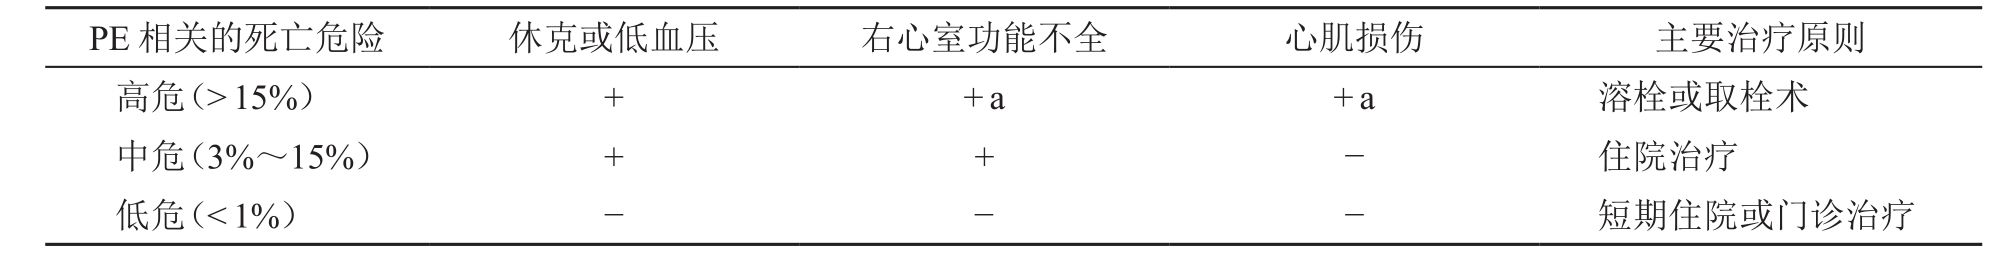
\includegraphics[width=6.65625in,height=0.84375in]{./images/Image00401.jpg}
\end{table}

注a:在出现休克或低血压时,不需要根据是否具有右心室功能不全或心肌损伤来判断高危患者

由于
PE的症状和体征均缺乏特异性,还可同时见于其他多种疾病,故人们常称PE为具有多种临床表现的潜在致死性疾病,因此PE应与下述常见疾病进行鉴别:冠心病、急性冠脉综合征、心肌炎、肺炎、胸膜炎、主动脉夹层、支气管哮喘、肺不张、慢性阻塞性肺气肿、原发性肺动脉高压及急性呼吸窘迫综合征(ARDS)等。在临床实践过程中,如熟知PE的临床表现特点,并将PE作为鉴别诊断的主要考虑内容,就会大大减少PE的误诊率及漏诊率。

\subsection{治疗}

\subsubsection{急性PE的治疗}

\hypertarget{text00278.htmlux5cux23CHP9-8-3-1-1}{}
(一) 一般性治疗

1.绝对卧床休息 2~3周,保持大便通畅,避免用力,以防血栓脱落。

2.密切监测患者的生命体征 ,动态监测心电图、动脉血气分析。

3.对症治疗 如胸痛、烦躁给予吗啡;缺氧予以吸氧;心衰按心衰治疗等。

4.对合并下肢深静脉血栓形成的患者应绝对卧床至抗凝治疗达到一定强度(保持国际标准化比值在2.0左右)方可,并应用抗生素控制下肢血栓性静脉炎和预防肺栓塞并发感染。

\hypertarget{text00278.htmlux5cux23CHP9-8-3-1-2}{}
(二) 溶栓治疗

溶栓治疗是高危
PE患者的一线治疗方案。对于出现休克或低血压的高危PE患者,只要不存在溶栓治疗绝对禁忌证,均应给予静脉溶栓治疗(Ⅰ类,证据级别A);而对于非高危患者,不建议常规进行溶栓治疗,只建议对中危患者选择性应用溶栓治疗(Ⅱb类,证据级别B);而对于低危患者,不建议行溶栓治疗(Ⅲ类,证据级别B)。

溶栓治疗可迅速溶解血栓,恢复栓塞区肺组织再灌注,减少肺动脉阻力,降低肺动脉高压,改善右心功能,可降低PE病死率及复发率。故溶栓治疗应越早越好,其溶栓的时间窗为PE起病48小时内即开始行溶栓治疗能够取得最大的疗效,但对于那些有症状的PE患者在起病6~14天内行溶栓治疗仍有一定作用。溶栓治疗主要并发症为出血。最严重的是颅内出血,发生率1\%~2\%,近半数死亡。用药前应充分评估出血的危险性,必要时应配血,作好输血准备。溶栓前宜留置外周静脉套管针,以方便溶栓中取血监测,避免反复穿刺血管。

\paragraph{溶栓治疗的绝对禁忌证}

①活动性内出血;②近期(14天内)自发性颅内出血。

\paragraph{溶栓治疗的相对禁忌证}

①2周内的大手术、分娩、器官活检或不能压迫止血部位的血管穿刺;②2个月内的缺血性卒中;③10天内的胃肠道出血;④15天内的严重创伤;⑤1个月内的神经外科或眼科手术;⑥难于控制的重度高血压(收缩压>
180mmHg,舒张压> 110mmHg);⑦近期曾行心肺复苏;⑧血小板< 100 ×
10\textsuperscript{9}
/L;⑨妊娠、分娩期;⑩其他有:感染性心内膜炎;严重肝、肾功能不全;糖尿病出血性视网膜病变;出血性疾病;动脉瘤;左心房血栓;年龄>
75岁等。

\paragraph{溶栓常用药物及治疗方案}

\hypertarget{text00278.htmlux5cux23CHP9-8-3-1-2-3-1}{}
(1) 链激酶:

负荷量25万U,静注30分钟,随后10万U/h持续静滴24小时。

\hypertarget{text00278.htmlux5cux23CHP9-8-3-1-2-3-2}{}
(2) 尿激酶:

①尿激酶12小时组:负荷量4400IU/kg,加生理盐水20ml,静注10分钟,随后2200IU/(kg•h),加入生理盐水250~500ml持续静滴12小时。②尿激酶2小时组:尿激酶2万IU/kg加入生理盐水100ml中持续静滴2小时。

\hypertarget{text00278.htmlux5cux23CHP9-8-3-1-2-3-3}{}
(3) 重组组织型纤溶酶原激活剂(rt-PA):

rt-PA 50~100mg加入注射用水100ml,持续静滴2小时。

\paragraph{各种溶栓方案比较}

链激酶溶栓效果不如尿激酶及rt-PA,而且易发生过敏反应,临床上已较少应用。目前国内常用溶栓方案为尿激酶2万IU/kg加入生理盐水100ml,持续静滴2小时及rt-PA
50~100mg加入注射用水100ml持续静滴2小时。为了对比常用溶栓方案的优劣,自2002年6月~2004年12月,由北京朝阳医院牵头观察246例PE病例不同溶栓方案治疗效果,发现尿激酶12小时组、尿激酶2小时组、rt-PA
50mg组及rt-PA
100mg组临床有效率分别为95.59\%、94.34\%、98.36\%及94\%,示rt-PA
50mg治疗组临床疗效最好。rt-PA具有纤维蛋白特异性,溶栓作用强,半衰期短,发挥作用快,能有效降低早期死亡率,减少了出血的不良反应,能够降低远期慢性血栓栓塞性肺动脉高压及下肢深静脉瓣功能不全后遗症的发生危险,用药后不会发生过敏反应。因此,溶栓治疗首选rt-PA方案。

\hypertarget{text00278.htmlux5cux23CHP9-8-3-1-3}{}
(三) 抗凝治疗

抗凝疗法为
PE的基本治疗方法,可有效防止血栓再度形成和复发,同时可使自身纤溶机制溶解已存在的血栓,有效阻止静脉血栓的进展。当临床疑诊PE时,即可予以抗凝治疗。常用的抗凝药物为肝素、低分子肝素及华法林,在治疗初期先用肝素或低分子肝素。一般来讲普通肝素、低分子量肝素至少应用5天,直到临床症状稳定方可停药。对于大块PE、髂静脉及(或)股静脉血栓患者,约需用至10天或者更长时间然后以华法林维持治疗。目前已研制成功新型抗凝药物:有磺达肝癸钠和利伐沙班等药物,为选择性Ⅹa因子抑制剂,临床上用于预防骨科术后静脉血栓形成。

当使用尿激酶、链激酶溶栓时不主张同时使用肝素治疗;但以rt-PA溶栓时,当rt-PA注射结束后,则必须应用肝素治疗。溶栓治疗结束后,应每2~4小时测定一次凝血酶原时间(PT)或活化部分凝血活酶时间(APTT),当其水平降至正常值的1.5~2倍时,即应开始规范的肝素治疗。

\paragraph{抗凝治疗绝对禁忌证}

①脑出血、消化系统出血急性期;②恶性肿瘤;③动静脉畸形。

\paragraph{抗凝治疗相对禁忌证}

①既往有出血性疾病;②血压未控制≥180/110mmHg;③2周内的大手术、创伤、活组织检查;④产后;⑤严重肝、肾功能不全。

\paragraph{抗凝药物用法}

\hypertarget{text00278.htmlux5cux23CHP9-8-3-1-3-3-1}{}
(1) 普通肝素(UFH):

首剂给予负荷剂量3000~5000IU或按80IU/kg静脉注射,继之以18IU/(kg•h)持续静脉滴注。抗凝必须充分,否则将严重影响疗效。在开始治疗后的最初24小时内,每4~6小时测定APTT,依APTT来调整肝素的用量,尽快使APTT达到并维持于正常值的1.5~2.0倍,当达到稳定治疗水平以后可每日上午检测APTT一次即可。肝素亦可用皮下注射方式给药,一般先予静注负荷量3000~5000IU,然后按250IU/kg剂量每12小时皮下注射1次。调节注射剂量,使注射后6~8小时的APTT达到治疗水平。肝素一般用7~10天。因可能会引起肝素诱导的血小板减少症(HIT),在使用UFH时,第1周每1~2天、第2周起每3~4天必须复查血小板计数一次,如出现血小板迅速或持续降低达30\%以上,或血小板计数<
100 × 10\textsuperscript{9}
/L,需及时停用UFH,一般在肝素停用后10天左右,血小板可逐渐恢复。在应用肝素过程中如发生大出血,可用全量鱼精蛋白对抗,即1mg鱼精蛋白对抗100IU肝素。

\hypertarget{text00278.htmlux5cux23CHP9-8-3-1-3-3-2}{}
(2) 低分子肝素(LMWH):

LMWH具有生物利用度好、无须检测APTT和调整剂量、HIT发生率低、安全等优点。国内常用的LMWH有:达肝素(法安明,100U/kg)、依诺肝素(克赛,100U/kg)和那屈肝素(速避凝,0.01ml/kg),均为每日2次皮下注射,最短用药时间7~10天。由于LMWH由肾脏清除,对于肾功能不全,尤为肌酐清除率<
30ml/min者慎用,而应选用UFH治疗。

\hypertarget{text00278.htmlux5cux23CHP9-8-3-1-3-3-3}{}
(3) 华法林:

为目前常用的口服抗凝剂,华法林是一种维生素K拮抗剂,它通过抑制依赖维生素K凝血因子(Ⅱ、Ⅶ、Ⅸ、Ⅹ)的合成而发挥抗凝作用,以预防PE的复发及静脉血栓的形成。由于华法林起效时间为2~3天,因此应于UFH(或LMWH)停药前3~4天开始服用,初始剂量为2.5~3.0mg/d,依国际标准化比值(INR)来调整华法林剂量,服华法林抗凝目标INR范围在2.0~3.0之间,服用华法林的并发症主要是出血,故服用华法林监测INR是十分重要的。初始服用华法林因INR未达标,故需每日监测INR,达标后头2周监测2~3次,以后如INR趋于稳定,则每周测一次,以后半月查一次INR,如INR均趋于稳定可4周查一次INR。

服用华法林时应注意以下情况:①华法林代谢受一些药物及食物影响而影响其清除:可使华法林抗凝作用增强的药物有阿司匹林、保泰松、西咪替丁、甲苯磺丁脲、奎尼丁、丙米嗪、头孢哌酮、头孢唑林、头孢噻吩、头孢曲松、红霉素、甲硝唑、磺胺类、环丙沙星、氧氟沙星、四环素、氟康唑、伊曲康唑、胺碘酮、普罗帕酮、三环类抗抑郁药、维生素E、丹参、当归等。可使华法林抗凝作用减弱的药物有苯妥英钠、苯巴比妥、维生素K、利福平、螺内酯、卡马西平、硫糖铝、人参、辅酶Q\textsubscript{10}
、抗甲状腺素药物等。绿叶蔬菜及绿茶也可降低华法林疗效。②华法林可透过胎盘影响胎儿致畸形,故禁用妊娠妇女,分娩后可用华法林,因母乳中华法林代谢物不具有抗凝作用。③华法林剂量大或INR
>
3.0时易发生出血,发生率6\%,对于轻~中度出血者可用维生素K拮抗。④华法林抗凝治疗的时间应因人而异,部分病例的危险因素可短期内消除,如口服雌激素、短期制动、创伤和手术等,抗凝治疗3个月即可;对于栓子来源不明的首发病例,给予抗凝治疗至少6个月;对于高危险因素的PE,如合并恶性肿瘤、复发性静脉血栓栓塞症、特发性或合并凝血因子异常的深静脉血栓形成致PE者,并发肺心病或肺动脉高压者需长期或终身抗凝治疗。

\hypertarget{text00278.htmlux5cux23CHP9-8-3-1-4}{}
(四) 肺动脉血栓摘除术

由于大块血栓所致
PE急性期死亡率达32\%,其中发病1小时内死亡达11\%,死因为猝死、休克及呼吸循环衰竭。因此对于大块PE患者,肺动脉血栓摘除术是迅速有效改善呼吸循环功能障碍的有效方法。其适应证:①急性大面积PE;②血流动力学不稳定,尤为伴循环衰竭(右心衰竭)或休克者;③肺动脉主干、主要分支完全堵塞,且有溶栓治疗禁忌证或溶栓等内科治疗无效的患者;④训练有素的介入治疗梯队。

\hypertarget{text00278.htmlux5cux23CHP9-8-3-1-5}{}
(五) 外科疗法

急性大块
PE经溶栓或肺动脉血栓摘除术等方法无效时可考虑行外科肺动脉直接取栓术,其手术风险较大,死亡率高。

\subsubsection{深静脉血栓形成的治疗}

由于70\%~90\%的PE栓子来源于深静脉血栓形成的栓子脱落,其中90\%以上来源于下肢深静脉及盆腔静脉血栓,故对于急性PE治疗同时必须兼顾深静脉血栓形成的治疗,否则PE易复发。

\hypertarget{text00278.htmlux5cux23CHP9-8-3-2-1}{}
(一) 一般性治疗

1.卧床2~3周,以防止血栓脱落。

2.患肢抬高 消肿促进血液循环。

3.抗感染 主要为G\textsuperscript{+} 菌,应用相应抗生素。

4.对症治疗。

\hypertarget{text00278.htmlux5cux23CHP9-8-3-2-2}{}
(二) 特殊治疗

\paragraph{肝素及华法林抗凝治疗}

方法同PE,疗程一般为6~12个月。

\paragraph{溶栓治疗}

方法同PE,并非常规应用,需个体化考虑。

\paragraph{取栓}

适用于抗凝及溶栓治疗疗效差,病情进展的病例。

\paragraph{下腔静脉滤器}

下腔深静脉血栓形成为PE重要的血栓来源,为防止血栓脱落及PE再发,在下肢放置下腔静脉滤器。因滤器只能预防肺栓塞复发,并不能治疗深静脉血栓形成,因此需严格掌握适应证,其适应证:①下肢近端静脉血栓,但抗凝治疗禁忌或抗凝治疗出现并发症者;②下肢近端静脉大块血栓溶栓治疗前;③经充分抗凝治疗后PE复发者;④伴有血流动力学不稳定的大块PE;⑤行导管介入治疗或肺动脉血栓剥脱术者;⑥伴严重肺动脉高压或肺源性心脏病患者。近些年来研究表明,植入永久型滤器后能减少PE的发生,但并发症发生率较高。早期滤器植入部位血栓形成的发生率为10\%,晚期DVT发生率约20\%,5年闭塞率约22\%,9年闭塞率约33\%。为避免腔静脉滤器长期留置体内带来的血栓并发症,可选择植入可回收滤器,能有效预防PE再发。待下肢静脉血栓消失或无血栓脱落风险时,可考虑在12~14天内将腔静脉滤器回收取出。

\subsection{慢性血栓栓塞性肺动脉高压}

为肺动脉内反复栓塞及血栓形成致肺血管阻力增加,表现为栓塞性肺动脉高压及右心功能不全。发病多隐匿、缓慢。内科多为对症治疗,无特异治疗方法,肺移植术及肺动脉血栓内膜剥脱术为主要治疗方法。

\protect\hypertarget{text00279.html}{}{}

\hypertarget{text00279.htmlux5cux23CHP9-8-5}{}
参 考 文 献

1.
急性肺血栓栓塞症诊断治疗中国专家共识.中国医师协会心血管内科医师分会,中国老年医学会心血管病专业委员会,中国医师协会循证医学专业委员会.心血管疾病防治指南与共识2009

2. Kenneth E,Wood DO. Major pulmonary embolism:review of a
pathophysiologic approach to the golden hour of hemodynamically
significant pulmonary embolism. Chest,2002,121:877-905

3. 荆志成
,邓可武.急性肺动脉血栓栓塞症的溶栓治疗.中华医学杂志,2004,84:1932-1934

4. Harry R,Baller Giancarlo Agnelli,Russel D Hull,et al.
Antithrobotic therapy for venous thromboembolic disease:the Seventy
ACCP conference on antithrombotic and thrombolytic therapy.
Chest,2004,126:401s-428s

5. Adam Torbicki,Chairperson,Arnaud Perrier,et al. Guidelines on the
diagnosis and management of acute pulmonary embolism:The Task Force for
the Diagnosis and Management of Acute Pulmonary Embolism of the European
Society of Cardiology(ESC).European Heart Journal,2008,9:2276-2315

\protect\hypertarget{text00280.html}{}{}

